\documentclass[12pt, a4paper]{report}

\usepackage[italian]{babel}

\usepackage[tmargin=3cm,rmargin=1in,lmargin=1in,margin=0.85in,bmargin=3cm]{geometry}
\usepackage{amsmath,amsfonts,amsthm,amssymb,mathtools}
\usepackage{bookmark}
\usepackage{enumitem}
\usepackage{hyperref}
\hypersetup{
	colorlinks=true,
  allcolors=fg,
	bookmarksnumbered=true,
	bookmarksopen=true
}
\usepackage[most,many,breakable]{tcolorbox}
\usepackage{xcolor}
\usepackage{algorithm}
\usepackage{algpseudocode}
\usepackage{caption}
\usepackage{subcaption}
\usepackage{float}
\usepackage{tikz}
\usepackage{tikz-cd}
\usepackage{tikzsymbols}
\usetikzlibrary{patterns, shapes.misc}
\usepackage{xpatch}% to patch \cancel
\usepackage[bottom]{footmisc}
\usepackage{graphbox}

\algdef{SE}[DOWHILE]{Do}{DoWhile}{\algorithmicdo}[1]{\algorithmicwhile\ #1}%


\definecolor{bg}{HTML}{F2F2F2}
\definecolor{fg}{HTML}{282828}

\setlength{\parindent}{0pt}

% change default chapter distance
\makeatletter
% --- Patch \chapter
\patchcmd{\@makechapterhead}{50\p@}{\chapheadtopskip}{}{}% Space from top of page to CHAPTER X
\patchcmd{\@makechapterhead}{20\p@}{\chapheadsep}{}{}% Space between CHAPTER X and CHAPTER TITLE
\patchcmd{\@makechapterhead}{40\p@}{\chapheadbelowskip}{}{}% Space between CHAPTER TITLE and text
% --- Patch \chapter*
\patchcmd{\@makeschapterhead}{50\p@}{\chapheadtopskip}{}{}% Space from top of page to CHAPTER TITLE
\patchcmd{\@makeschapterhead}{40\p@}{\chapheadbelowskip}{}{}% SPace between CHAPTER TITLE and text
\makeatother
% Set new lengths
\newlength{\chapheadtopskip}\setlength{\chapheadtopskip}{0pt}
\newlength{\chapheadsep}\setlength{\chapheadsep}{15pt}
\newlength{\chapheadbelowskip}\setlength{\chapheadbelowskip}{25pt}

% deliminators
\DeclarePairedDelimiter{\abs}{\lvert}{\rvert}
\DeclarePairedDelimiter{\norm}{\lVert}{\rVert}

\DeclarePairedDelimiter{\ceil}{\lceil}{\rceil}
\DeclarePairedDelimiter{\floor}{\lfloor}{\rfloor}
\DeclarePairedDelimiter{\round}{\lfloor}{\rceil}

\let\oldleq\leq
\let\oldgeq\geq
\renewcommand{\leq}{\leqslant}
\renewcommand{\geq}{\geqslant}

\usepackage{titletoc}
\contentsmargin{0cm}
\titlecontents{part}[-1pc]
{\addvspace{50pt}%
	\begin{tikzpicture}[remember picture, overlay]%
		\draw[fill=fg!85,draw=fg!85] (-4.5,-0.2) rectangle (-0.15,0.55);%
		\pgftext[left,x=-1.6cm,y=0.15cm]{\color{bg}\Large Part}%
	\end{tikzpicture}\color{fg}\large}
{}
{}
{}
\titlecontents{chapter}[5pc]
{\addvspace{30pt}%
	\begin{tikzpicture}[remember picture, overlay]%
		\draw[fill=fg!85,draw=fg!85] (-3.6,-0.2) rectangle (-0.12,0.55);%
		\pgftext[left,x=-3.5cm,y=0.15cm]{\color{bg}\Large Chapter\ \thecontentslabel}%
	\end{tikzpicture}\color{fg}\large}%
{}
{}
{\;\titlerule\;\large Page \thecontentspage
	\begin{tikzpicture}[remember picture, overlay]
		\draw[fill=fg,draw=fg] (4pt,0.2pt) rectangle (4,0.2pt);
	\end{tikzpicture}}%
\titlecontents{section}[5pc]
{\addvspace{2pt}}
{\contentslabel[\thecontentslabel]{2pc}}
{}
{\hfill\small \thecontentspage}
[]
\titlecontents{subsection}[5pc]
{\addvspace{2pt}}
{\scriptsize$\bullet$\quad\small}
{}
{\hfill\small}
[]

\makeatletter
\renewcommand{\tableofcontents}{%
	\chapter*{%
	  \vspace*{-20\p@}%
	  \begin{tikzpicture}[remember picture, overlay]%
		  \pgftext[right,x=16.7cm,y=0.2cm]{\color{fg!85}\Huge \contentsname}%
		  \draw[fill=fg!85,draw=fg!85] (14.6,-0.65) rectangle (20,1);%
		  \clip (14.6,-0.65) rectangle (20,1);
		  \pgftext[right,x=16.7cm,y=0.2cm]{\color{bg}\Huge \contentsname}%
	  \end{tikzpicture}}%
	\@starttoc{toc}}
\makeatother

\usepackage[italian]{babel}

\title{\Huge{Implementazione distribuita dell'algoritmo Flood-Fill}}
\author{\Large{\textit{Tam Gabriele, Merlo Filippo}}}
\date{\today}

\begin{document}

\maketitle

\newpage
\pdfbookmark[section]{\contentsname}{toc}
\tableofcontents
\pagebreak

\begin{abstract} L'algoritmo Flood-Fill \`e una tecnica utilizzata per ricolorare aree connesse in strutture bidimensionali, comunemente applicato in grafica computerizzata. L'obiettivo di questo progetto \`e l'implementazione distribuita dell'algoritmo, con una rappresentazione dove ogni pixel di un'immagine \`e trattato come un nodo di una rete distribuita. In questo contesto, emergono sfide legate alla comunicazione tra nodi, alla consistenza dello stato, alla gestione delle richieste concorrenti e alla tolleranza ai guasti.

Nel documento viene proposto un approccio basato su una partizione dei nodi in cluster, gestiti da nodi leader, e su una rete overlay tra leader per facilitare operazioni di merge e coordinamento. Viene implementato un sistema che garantisce scalabilit\`a, robustezza e consistenza utilizzando un time-server che gestisce i timestamp per l'ordinamento degli eventi e un database condiviso per la sincronizzazione globale. Inoltre, il sistema \`e progettato per essere resiliente ai guasti, con meccanismi di elezione di nuovi leader e recupero dei nodi. I risultati mostrano che la soluzione proposta \`e efficiente e adatta a reti di grandi dimensioni. \end{abstract}

\chapter{Introduzione}

In questo capitolo viene descritto il problema principale affrontato dal progetto, insieme a una panoramica della soluzione proposta. L'obiettivo \`e sviluppare una versione distribuita dell'algoritmo \emph{Flood-Fill}, che permette di ricolorare aree connesse in una struttura bidimensionale, come un'immagine digitale, dove ogni pixel \`e rappresentato da un nodo della rete distribuita. Questo scenario introduce sfide legate alla comunicazione tra nodi, alla gestione delle operazioni concorrenti e alla tolleranza ai guasti, tutti aspetti che devono essere gestiti in modo efficiente.

\section{Descrizione del problema}

Il problema consiste nel ricolorare un'area connessa di una matrice bidimensionale $img[N][M]$, dove ogni elemento $img[i][j]$\footnote{con $0 \le i < N$ e $0 \le j < M$} rappresenta il colore di un pixel in posizione $(i,j)$. Dato un pixel iniziale in posizione \texttt{(x, y)} e un nuovo colore \texttt{newColor}, l'obiettivo \`e cambiare il colore del pixel selezionato e di tutti i pixel adiacenti che condividono lo stesso colore iniziale con \texttt{newColor} (vedi Fig.~\ref{fig:esempio_nodi}). Questa ricolorazione deve propagarsi attraverso nodi adiacenti, in tutte le direzioni (orizzontale, verticale, diagonale).

\begin{figure}[H]
    \captionsetup{justification=centering, margin=2cm}
    \centering
    \begin{subfigure}{0.48\textwidth}
        \captionsetup{justification=centering, margin=1cm}
        \centering
        \begin{tikzpicture}
    \fill[black!30] (1, 5) rectangle ++(1,1);
    \fill[black!30] (3, 5) rectangle ++(1,1);
    \fill[black!30] (2, 4) rectangle ++(1,1);
    \fill[black!30] (2, 6) rectangle ++(1,1);
    \fill[black!30] (3, 6) rectangle ++(1,1);
    \fill[black!30] (3, 4) rectangle ++(1,1);
    \fill[black!30] (1, 6) rectangle ++(1,1);
    \fill[black!30] (1, 4) rectangle ++(1,1);

    \fill[red!30] (2, 5) rectangle ++(1,1);

    \draw[thick, black] (1, 5) rectangle ++(1,1);
    \draw[thick, black] (3, 5) rectangle ++(1,1);
    \draw[thick, black] (2, 4) rectangle ++(1,1);
    \draw[thick, black] (2, 6) rectangle ++(1,1);
    \draw[thick, black] (3, 6) rectangle ++(1,1);
    \draw[thick, black] (3, 4) rectangle ++(1,1);
    \draw[thick, black] (1, 6) rectangle ++(1,1);
    \draw[thick, black] (1, 4) rectangle ++(1,1);

    \draw[thick, red] (2, 5) rectangle ++(1,1);
    
    % Draw the grid and add colored letters
    \node[fill=red!60, text=white, font=\bfseries] at (0.5, 6.5) {R}; 
    \node[fill=red!60, text=white, font=\bfseries] at (1.5, 6.5) {R}; 
    \node[fill=blue!60, text=white, font=\bfseries] at (2.5, 6.5) {B}; 
    \node[fill=cyan!60, text=white, font=\bfseries] at (3.5, 6.5) {C}; 
    \node[fill=cyan!60, text=white, font=\bfseries] at (4.5, 6.5) {C};
    
    \node[fill=red!60, text=white, font=\bfseries] at (0.5, 5.5) {R}; 
    \node[fill=red!60, text=white, font=\bfseries] at (1.5, 5.5) {R}; 
    \node[fill=blue!60, text=white, font=\bfseries] at (2.5, 5.5) {B}; 
    \node[fill=cyan!60, text=white, font=\bfseries] at (3.5, 5.5) {C}; 
    \node[fill=cyan!60, text=white, font=\bfseries] at (4.5, 5.5) {C};
    
    \node[fill=red!60, text=white, font=\bfseries] at (0.5, 4.5) {R}; 
    \node[fill=red!60, text=white, font=\bfseries] at (1.5, 4.5) {R}; 
    \node[fill=blue!60, text=white, font=\bfseries] at (2.5, 4.5) {B};  % Nodo centrale
    \node[fill=green!60, text=white, font=\bfseries] at (3.5, 4.5) {G}; 
    \node[fill=green!60, text=white, font=\bfseries] at (4.5, 4.5) {G};
    
    \node[fill=red!60, text=white, font=\bfseries] at (0.5, 3.5) {R}; 
    \node[fill=red!60, text=white, font=\bfseries] at (1.5, 3.5) {R}; 
    \node[fill=blue!60, text=white, font=\bfseries] at (2.5, 3.5) {B}; % Vicino dello stesso colore
    \node[fill=green!60, text=white, font=\bfseries] at (3.5, 3.5) {G}; 
    \node[fill=green!60, text=white, font=\bfseries] at (4.5, 3.5) {G};
    
    \node[fill=blue!60, text=white, font=\bfseries] at (0.5, 2.5) {B}; 
    \node[fill=blue!60, text=white, font=\bfseries] at (1.5, 2.5) {B}; % Vicino dello stesso colore
    \node[fill=blue!60, text=white, font=\bfseries] at (2.5, 2.5) {B}; % Vicino dello stesso colore
    \node[fill=green!60, text=white, font=\bfseries] at (3.5, 2.5) {G}; 
    \node[fill=green!60, text=white, font=\bfseries] at (4.5, 2.5) {G};
\end{tikzpicture}
        \caption{L'area evidenziata in grigio sono i nodi adiacenti.}
        \label{fig:nodi_adiacenti}
    \end{subfigure}
    \hfill
    \begin{subfigure}{0.48\textwidth}
        \captionsetup{justification=centering, margin=1cm}
        \centering
        \begin{tikzpicture}
    \fill[orange!30] (2, 6) rectangle ++(1,1);
    \fill[red!30] (2, 5) rectangle ++(1,1);
    \fill[orange!30] (2, 4) rectangle ++(1,1);
    \fill[orange!30] (2, 3) rectangle ++(1,1);
    \fill[orange!30] (2, 2) rectangle ++(1,1);
    \fill[orange!30] (1, 2) rectangle ++(1,1);
    \fill[orange!30] (0, 2) rectangle ++(1,1);

    \draw[thick, black] (2, 6) rectangle ++(1,1);
    \draw[thick, black] (2, 4) rectangle ++(1,1);
    \draw[thick, black] (2, 3) rectangle ++(1,1);
    \draw[thick, black] (2, 2) rectangle ++(1,1);
    \draw[thick, black] (1, 2) rectangle ++(1,1);
    \draw[thick, black] (0, 2) rectangle ++(1,1);
    
    \draw[thick, red] (2, 5) rectangle ++(1,1);

    
    % Draw the grid and add colored letters
    \node[fill=red!60, text=white, font=\bfseries] at (0.5, 6.5) {R}; 
    \node[fill=red!60, text=white, font=\bfseries] at (1.5, 6.5) {R}; 
    \node[fill=blue!60, text=white, font=\bfseries] at (2.5, 6.5) {B}; 
    \node[fill=cyan!60, text=white, font=\bfseries] at (3.5, 6.5) {C}; 
    \node[fill=cyan!60, text=white, font=\bfseries] at (4.5, 6.5) {C};
    
    \node[fill=red!60, text=white, font=\bfseries] at (0.5, 5.5) {R}; 
    \node[fill=red!60, text=white, font=\bfseries] at (1.5, 5.5) {R}; 
    \node[fill=blue!60, text=white, font=\bfseries] at (2.5, 5.5) {B}; 
    \node[fill=cyan!60, text=white, font=\bfseries] at (3.5, 5.5) {C}; 
    \node[fill=cyan!60, text=white, font=\bfseries] at (4.5, 5.5) {C};
    
    \node[fill=red!60, text=white, font=\bfseries] at (0.5, 4.5) {R}; 
    \node[fill=red!60, text=white, font=\bfseries] at (1.5, 4.5) {R}; 
    \node[fill=blue!60, text=white, font=\bfseries] at (2.5, 4.5) {B};  % Nodo centrale
    \node[fill=green!60, text=white, font=\bfseries] at (3.5, 4.5) {G}; 
    \node[fill=green!60, text=white, font=\bfseries] at (4.5, 4.5) {G};
    
    \node[fill=red!60, text=white, font=\bfseries] at (0.5, 3.5) {R}; 
    \node[fill=red!60, text=white, font=\bfseries] at (1.5, 3.5) {R}; 
    \node[fill=blue!60, text=white, font=\bfseries] at (2.5, 3.5) {B}; % Vicino dello stesso colore
    \node[fill=green!60, text=white, font=\bfseries] at (3.5, 3.5) {G}; 
    \node[fill=green!60, text=white, font=\bfseries] at (4.5, 3.5) {G};
    
    \node[fill=blue!60, text=white, font=\bfseries] at (0.5, 2.5) {B}; 
    \node[fill=blue!60, text=white, font=\bfseries] at (1.5, 2.5) {B}; % Vicino dello stesso colore
    \node[fill=blue!60, text=white, font=\bfseries] at (2.5, 2.5) {B}; % Vicino dello stesso colore
    \node[fill=green!60, text=white, font=\bfseries] at (3.5, 2.5) {G}; 
    \node[fill=green!60, text=white, font=\bfseries] at (4.5, 2.5) {G};
\end{tikzpicture}
        \caption{L'area evidenziata in giallo sono i nodi del cluster.}
        \label{fig:nodi_cluster}
    \end{subfigure}
    \caption{A partire dal nodo scelto (evidenziato di rosso), si mostrano i suoi nodi adiacenti (\ref{fig:nodi_adiacenti}) e quelli del cluster (\ref{fig:nodi_cluster}).}
    \label{fig:esempio_nodi}
\end{figure}


Ogni nodo della rete \`e responsabile di un pixel e collabora con i nodi adiacenti per completare l'operazione di ricolorazione.

\section{Terminologia}

Per una migliore comprensione e per evitare ambiguit\`a, vengono definiti alcuni termini chiave:

\begin{itemize}[label=]
    \item \textbf{Nodo}: un processo autonomo nella rete, responsabile di un singolo pixel dell'immagine.
    \item \textbf{Colore}: la propriet\`a associata a ciascun nodo, che rappresenta lo stato corrente (colore) del pixel.
    \item \textbf{Nodi adiacenti}: i nodi che si trovano in posizioni fisicamente adiacenti nella matrice, ovvero collegati orizzontalmente, verticalmente o diagonalmente.
    \item \textbf{Cluster}: un gruppo di nodi, i quali condividono lo stesso colore e sono connessi tra loro. Nel nostro approccio di soluzione, i cluster vengono gestiti a livello locale per ottimizzare le operazioni di ricolorazione.
    \item \textbf{Nodo Leader}: il nodo designato all'interno di un cluster per coordinare le operazioni globali, come l'avvio delle ricolorazioni e la fusione con altri cluster.
    \item \textbf{Ricolorazione/Cambio colore}: l'operazione di aggiornamento del colore di un cluster.
    \item \textbf{Unione/Merge di cluster}: l'unione di due o pi\`u cluster in uno singolo, nel caso in cui questi siano adiacenti e condividano lo stesso colore. Quest'operazione avviene in seguito a un cambio colore.
\end{itemize}

\section{Struttura complessiva dell'implementazione}

Il sistema \`e strutturato come una rete di nodi, i quali sono organizzati in cluster basati sul colore condiviso. Ogni cluster \`e gestito da un \emph{nodo leader}, il quale si occupa di coordinare le operazioni sia interne che esterne al cluster: la gestione delle operazioni distribuite richiede una comunicazione efficiente, che \`e garantita tramite una rete overlay tra i leader dei cluster e l'uso di un server centrale per mantenere lo stato globale del sistema.

\section{Caratteristiche del sistema distribuito}

Il sistema implementa diverse funzionalit\`a proprie dei sistemi distribuiti:
\begin{itemize}
    \item \textbf{Trasparenza nella comunicazione}: ogni nodo comunica direttamente con i nodi adiacenti, o con il leader del cluster, senza necessit\`a di conoscere la topologia completa.
    \item \textbf{Consistenza}: la consistenza globale del sistema \`e garantita tramite l'associazione di ogni operazione a un record evento. Gli eventi garantiscono sia una corretta gestione delle operazioni, tramite l'ordinamento per \textbf{timestamp} ed \textbf{id}, sia la loro archiviazione tramite logging. Vengono evitati cos\`i possibili conflitti dovuti alla concorrenza.
    \item \textbf{Tolleranza ai guasti}: meccanismi di failover assicurano che il sistema possa continuare a funzionare anche in caso di guasti di singoli nodi (sia normali che leader). I processi di ogni nodo vengono monitorati in caso di arresti inaspettati e riavviati immediatamente.
\end{itemize}

\section{Algoritmi implementati}

Il sistema utilizza vari algoritmi per garantire la corretta esecuzione dell'algoritmo distribuito di Flood-Fill:
\begin{itemize}
    \item \textbf{Algoritmo di cambio colore}: i nodi comunicano al leader del cluster la volont\`a di cambiare colore. Quest'ultimo gestisce le richieste per mezzo di una coda e comunica ognuna al server per avere la conferma per procedere con la ricolorazione locale. Il server viene coinvolto sia per garantire la consistenza, sia per evitare comportamenti inaspettati del sistema nel caso di operazioni concorrenti in cluster differenti.
    \item \textbf{Algoritmo di merge dei cluster}: quando due cluster adiacenti condividono lo stesso colore (in seguito a operazioni di cambio colore), i leader coinvolti ed il server collaborano per eseguire l'operazione di merge.
    \item \textbf{Algoritmo di gestione dei fallimenti}: include procedure per la rielezione dei leader e la gestione dei nodi disconnessi o falliti.
\end{itemize}

\section{Piano di test}

Il sistema sar\`a testato simulando scenari di ricolorazione su immagini di grandi dimensioni: i test valuteranno la robustezza del sistema in differenti situazioni di concorrenza (concorrenza di cambio colore intra/extra-cluster e del merge di cluster) ed anche in presenza di guasti di nodi. L'attenzione sar\`a posta sulla consistenza delle operazioni distribuite.

\section{Programma di sviluppo}

Il progetto si articola in diverse fasi:
\begin{enumerate}
    \item \textbf{Fase di progettazione}: definizione dell'architettura del sistema e degli algoritmi distribuiti.
    \item \textbf{Fase d'implementazione}: sviluppo del codice del sistema distribuito nel linguaggio Erlang e scrittura del frontend e degli script di test in Python.
    \item \textbf{Fase di testing}: esecuzione di test per verificare il corretto funzionamento del sistema, nonch\`e valutazione delle prestazioni e della scalabilit\`a del sistema sviluppato.
\end{enumerate}

\chapter{Analisi}\label{chapter:analisi}

In questo capitolo vengono descritti nel dettaglio i requisiti funzionali e non funzionali di una soluzione per l'implementazione distribuita dell'algoritmo \emph{Flood-Fill}. Questi requisiti guidano lo sviluppo del sistema, specificando le funzionalit\`a richieste e le qualit\`a desiderabili, insieme alle assunzioni e ai vincoli considerati durante l'implementazione.

\section{Requisiti funzionali}

I requisiti funzionali definiscono le operazioni principali che il sistema deve offrire, specificando come devono essere gestiti input e output, e l'effetto atteso per ogni funzione.

\begin{enumerate}
    \item \textbf{Operazione di colorazione distribuita}: il sistema deve permettere a un nodo di iniziare un'operazione di ricolorazione, propagando il nuovo colore a tutti i nodi adiacenti che condividono lo stesso colore iniziale.

    \item \textbf{Gestione di richieste concorrenti}: il sistema deve essere in grado di gestire pi\`u richieste di ricolorazione simultanee provenienti da nodi diversi, garantendo un comportamento deterministico e la corretta risoluzione dei conflitti.

    \item \textbf{Comunicazione tra nodi}: i nodi devono essere in grado di scambiarsi messaggi con i loro vicini adiacenti per la sincronizzazione dello stato e la coordinazione delle operazioni. Ogni nodo deve mantenere aggiornate le informazioni relative ai vicini e al leader del proprio cluster.

    \item \textbf{Unione di cluster}: quando due o pi\`u cluster adiacenti diventano dello stesso colore in seguito a ricolorazioni, il sistema deve unificarli in uno solo.

    \item \textbf{Tolleranza ai guasti}: il sistema deve essere in grado di gestire il fallimento di singoli nodi, sia leader che normali, garantendo che il resto del cluster continui a operare correttamente. Devono essere previsti meccanismi di failover per la rielezione dei leader.

    \item \textbf{Consistenza globale}: il sistema deve mantenere una consistenza globale dello stato, garantendo che tutti i nodi di un cluster condividano lo stesso colore dopo ogni operazione di cambio colore o merge.
\end{enumerate}

\newpage
\section{Requisiti non funzionali}\label{sec:requisiti_non_funzionali}

I requisiti non funzionali riguardano le qualit\`a desiderabili del sistema, tra cui prestazioni, sicurezza e tolleranza ai guasti. Essi descrivono le caratteristiche che devono essere garantite durante l'implementazione.

\begin{enumerate}
    \item \textbf{Scalabilit\`a}: il sistema deve essere in grado di supportare un elevato numero di nodi, mantenendo buone prestazioni anche con una rete distribuita estesa.

    \item \textbf{Efficienza delle comunicazioni}: il numero di messaggi scambiati tra i nodi deve essere minimizzato per evitare sovraccarichi di rete. Gli algoritmi di ricolorazione e unione devono utilizzare una comunicazione locale, limitata ai vicini diretti, salvo necessit\`a di sincronizzazione globale.

    \item \textbf{Robustezza e affidabilit\`a}: il sistema deve essere resiliente ai guasti e garantire il recupero rapido dopo il fallimento di uno o pi\`u nodi, inclusi i nodi leader. Deve essere possibile continuare le operazioni anche in caso di guasti isolati.

    \item \textbf{Consistenza}: il sistema deve garantire la consistenza dello stato anche in presenza di richieste concorrenti o di fallimenti.

\end{enumerate}

\section{Assunzioni e vincoli}

Le seguenti assunzioni e vincoli sono stati considerati per l'implementazione del sistema distribuito:

\begin{itemize}
    \item \textbf{Topologia della rete}: si assume che la rete sottostante sia affidabile, ossia che i messaggi inviati tra nodi adiacenti vengano consegnati correttamente entro un tempo limite ragionevole.

    \item \textbf{Fallimenti dei nodi}: si assume che i nodi possano fallire in modalit\`a \emph{crash}, ossia che possano smettere di funzionare senza comportamento bizantino (comportamenti non affidabili o malevoli).

    \item \textbf{Conoscenza locale}: ogni nodo ha una conoscenza locale limitata dei propri vicini e del leader del proprio cluster. Nessun nodo ha una visione globale dell'intera rete o di tutti i cluster.

    \item \textbf{Inizializzazione dei nodi}: al momento dell'avvio, ogni nodo conosce solo le proprie coordinate all'interno della matrice dell'immagine e il colore iniziale del pixel che rappresenta. La formazione dei cluster e la gestione della rete overlay avvengono durante la fase iniziale d'avvio del sistema.

\end{itemize}

\chapter{Progettazione del sistema}

In questo capitolo viene presentata la progettazione del sistema: verranno analizzate le possibili soluzioni, spiegando i vantaggi e gli svantaggi di ciascuna e successivamente verr\`a presentata la soluzione scelta, descrivendone architettura, componenti ed algoritmi utilizzati.

\section{Analisi delle possibili soluzioni}

Sono stati considerati due principali approcci:

\begin{enumerate}
    \item \textbf{Comunicazione diretta tra nodi}: nodi normali e leader comunicano direttamente tra loro per eseguire le operazioni di cambio colore e merge. Cluster adiacenti comunicano direttamente per mezzo dei propri leader.
    \item \textbf{Partizionamento del grafo e elezione di nodi leader}: il grafo viene suddiviso in cluster, ciascuno gestito dal proprio nodo leader che ne coordina operazioni (e.g. ricolorazione) ed organizzazione (e.g. fallimento di nodi, merge, $\ldots$).
\end{enumerate}

\subsubsection{1. Comunicazione diretta tra nodi}

\paragraph{Descrizione generale}
\begin{flushleft}
In questo approccio, ogni nodo mantiene informazioni locali e comunica direttamente con i nodi adiacenti. Quando un nodo cambia colore, l'operazione di ricolorazione viene unicamente propagata ai nodi adiacenti che condividono lo stesso colore, creando una diffusione a cascata.
\end{flushleft}

\paragraph{Vantaggi}

\begin{itemize}
    \item \textbf{Semplicit\`a}: l'implementazione \`e relativamente semplice poich\'e ogni nodo gestisce solo informazioni locali.
    \item \textbf{Assenza di punti singoli di fallimento}: non esistono nodi centrali il cui fallimento compromette l'intero sistema.
\end{itemize}

\paragraph{Svantaggi}

\begin{itemize}
    \item \textbf{Scalabilit\`a limitata}: l'elevato numero di messaggi scambiati pu\`o diventare insostenibile in reti di grandi dimensioni.
    \item \textbf{Concorrenza non deterministica}: difficolt\`a nel gestire richieste concorrenti in modo deterministico.
    \item \textbf{Gestione dei fallimenti complessa}: la mancanza di una visione globale rende difficile il recupero da guasti.
\end{itemize}

\subsubsection{2. Partizionamento del grafo e nodi leader}

\paragraph{Descrizione generale}
\begin{flushleft}
In questo approccio, il grafo \`e partizionato in cluster, ognuno dei quali \`e gestito dal proprio \textbf{nodo leader} responsabile della gestione dello stato e delle decisioni per il cluster. I nodi normali delegano le decisioni al leader, riducendo la complessit\`a locale.
\end{flushleft}
\paragraph{Vantaggi}

\begin{itemize}
    \item \textbf{Consistenza migliorata}: la centralizzazione delle decisioni nel leader migliora la consistenza del sistema.
    \item \textbf{Gestione efficiente della concorrenza}: il leader gestisce richieste concorrenti in modo ordinato.
    \item \textbf{Scalabilit\`a}: partizionando il grafo si riduce la complessit\`a in cluster pi\`u piccoli.
\end{itemize}

\paragraph{Svantaggi}

\begin{itemize}
    \item \textbf{Punti singoli di fallimento}: il fallimento del leader pu\`o compromettere il funzionamento del cluster.
    \item \textbf{Complessit\`a aggiuntiva}: l'implementazione di leader, algoritmi di elezione e meccanismi di consenso aggiungono complessit\`a.
    \item \textbf{Possibili colli di bottiglia}: il leader pu\`o diventare un collo di bottiglia in cluster molto attivi.
\end{itemize}

\section{Soluzione proposta}

In questo progetto \`e stato usato come base il secondo approccio appena presentato, il quale \`e stato arricchito di varie scelte implementative atte a limitare al minimo gli svantaggi della soluzione, senza intaccare i vantaggi di essa. L'idea della soluzione qui presentata \`e di trattare ogni cluster come un nodo in un grafo \emph{overlay}: ci\`o permette una gestione efficiente delle comunicazioni tra cluster, semplifica le operazioni di merge e cambio colore, e facilita la consistenza globale del sistema.

\subsection{Idea principale}

L'idea centrale della soluzione \`e la seguente:

\begin{itemize}
    \item \textbf{Trattamento dei cluster come nodi in un grafo overlay}: ogni cluster viene considerato come un singolo nodo in un grafo overlay, dove i nodi rappresentano i leader dei cluster e gli archi rappresentano le adiacenze tra cluster.
    \item \textbf{Comunicazione tra leader}: i nodi leader mantengono una lista dei leader adiacenti nel grafo overlay, permettendo comunicazioni dirette per le operazioni di merge e coordinamento.
    \item \textbf{Utilizzo di un server centrale per la sincronizzazione}: implementazione di un server condiviso per gestione, ordinamento e memorizzazione delle operazioni eseguite. Facilita la consistenza e la gestione delle operazioni concorrenti, fornendo al tempo stesso ridondanza sia delle operazioni eseguite (attraverso un file di log) sia dello stato globale della rete.
\end{itemize}

\subsection{Setup iniziale}\label{subsec:setup}

La fase di setup \`e fondamentale per l'inizializzazione dei parametri dei nodi e la costruzione dei cluster, i quali costituiranno il sistema distribuito. Poiché i nodi inizialmente conoscono solo informazioni su loro stessi, il processo di formazione dei cluster e la scoperta delle connessioni tra di essi viene suddiviso in tre fasi, ciascuna con uno scopo specifico:

\begin{itemize}
    \item \textbf{Fase 1: Scoperta dei vicini}
    \item \textbf{Fase 2: Formazione dei cluster}
    \item \textbf{Fase 3: Scoperta dei cluster adiacenti e costruzione della rete overlay}
\end{itemize}


Inizialmente ogni nodo conosce solo:
\begin{itemize}
    \item Le proprie coordinate \texttt{(x, y)} nell'immagine.
    \item Il proprio colore \texttt{color}, assegnato randomicamente da una palette predefinita oppure impostato dall'utente attraverso un file contente la lista dei colori.
\end{itemize}

\paragraph{Fase 1: Scoperta dei vicini}
Attraverso le coordinate del nodo, vengono calcolate le posizioni dei nodi adiacenti. Con queste vengono recuperati gli id dei nodi, i quali vengono salvati nella lista \textit{neighbors}.

\paragraph{Fase 2: Formazione dei cluster}
Per ogni nodo del sistema viene eseguito un algoritmo di scoperta dei nodi del cluster simile all'algoritmo BFS\footnote{Breadth-First Search}. Ad ogni nodo viene associata una variable \textit{Visited} inizialmente impostata a \texttt{False}. Sfruttando la lista \textit{neighbors} creata nella fase precedente, vengono ricorsivamente scoperti i nodi adiacenti tra loro che condividono lo stesso colore. L'algoritmo di visita termina quando non ci sono pi\`u vicini con colore uguale a quello del nodo di partenza. Ogni nodo che inizia l'algoritmo di visita diventa leader del cluster, mentre tutti i nodi scoperti saranno nodi normali che fanno parte del cluster. Ogni nodo del cluster viene salvato nella lista \textit{cluster\_nodes}.
    
\paragraph{Fase 3: Scoperta dei cluster adiacenti e creazione della rete overlay}
Nella terza ed ultima fase, viene costruita la lista dei cluster adiacenti, in cui ogni elemento della lista \`e una tripla del tipo \texttt{\{pid, colore, leader\}}. La lista (\textit{adj\_nodes}) viene costruita facendo la sottrazione della lista dei nodi del cluster (\textit{cluster\_nodes}) dalla lista cumulativa di tutti i vicini (\textit{neighbors}) di ogni nodo. La lista ottenuta \`e costituita da tutti i nodi che compongono il ``contorno'' del cluster, ovvero nodi vicini ma con colore diverso.
Infine per ogni nodo nella lista vengono prese le informazioni riguardo all'id del leader e il colore del cluster, rimuovendo possibili duplicati e salvando tutto nella lista \textit{adj\_clusters}.

\paragraph{Conclusione del setup}
Al termine delle 3 fasi di setup, ogni nodo non leader viene trasformato in nodo normale rimuovendo le informazioni non pi\`u necessarie, ma mantendendo solo
\begin{itemize}
    \item \texttt{pid}: l'id del processo nodo.
    \item \texttt{(x, y)}: le proprie coordinate.
    \item \texttt{leaderID}: l'identificatore del leader del proprio cluster.
    \item \texttt{neighbors}: la lista dei nodi fisicamente vicini (indipendentemente dal colore).
\end{itemize}
Al contrario, ogni leader comunica le informazioni del proprio cluster al server e quest'ultimo si occuper\`a di salvare lo stato globale del sistema.
Questo processo riduce l'overhead e ottimizza la memoria utilizzata dai nodi.

Il sistema \`e ora sincronizzato ed \`e pronto per entrare nella fase operativa.

\begin{figure}
    \centering
    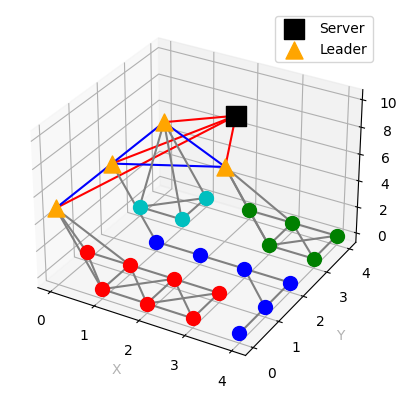
\includegraphics[width=0.5\linewidth]{images/setup/Esempio_Grafo_G.png}
    \caption{Esempio della struttura del sistema distribuito in una matrice di $5\times5$ pixel. Nel livello pi\`u basso sono presenti i nodi normali, colorati in base al cluster di appartenenza. Ogni cluster ha un leader, rappresentato da un triangolo arancione e sopraelevato rispetto ai nodi normali. I leader comunicano tra loro attraverso un overlay, mostrato con archi blu, e sono collegati al nodo server, rappresentato da un quadrato nero, mediante archi rossi.}
    \label{fig:enter-label}
\end{figure}

\paragraph{Complessit\`a della fase di setup}\label{par:complessita_setup}

Di seguito viene riportata l'analisi della complessit\`a delle due fasi.

\vspace{-5pt}
\begin{itemize}
    \item \textbf{Fase 1: Scoperta dei vicini}
    \vspace{-5pt}
    \begin{itemize}
      \item Per ogni nodo vengono calcolati i vicini usando la propria posizione, pertanto vengono eseguite $N \times M$ chiamate.
      \item Ciascuna chiamata ha complessit\`a $O(8)$, in quanto vi possono essere al massimo 8 vicini considerando orizzontale, verticale e diagonale.
      \item La complessit\`a totale della fase 1 \`e quindi $O(N \times M)$.
    \end{itemize}

    \item \textbf{Fase 2: Formazione dei cluster}
    \begin{itemize}
        \item Il server avvia l'algoritmo per formare i cluster, scorrendo l'immagine da sinistra a destra e dall'alto verso il basso.
        \item Per ogni nodo non ancora visitato, viene avviato un algoritmo di scoperta che include tutti i nodi adiacenti con lo stesso colore.
        \item La complessit\`a dell'algoritmo per ogni cluster \`e lineare rispetto al numero di nodi nel cluster, ossia $O(k)$, dove $k$ \`e il numero di nodi del cluster.
        \item Poiché ogni nodo dell'immagine viene visitato esattamente una volta, la complessit\`a totale della formazione dei cluster \`e $O(N \times M)$, dove $N \times M$ rappresenta il numero totale di nodi nell'immagine.
    \end{itemize}

    \item \textbf{Fase 3: Scoperta dei cluster adiacenti}
    \begin{itemize}
        \item Dopo la formazione dei cluster, i leader inviano richieste ai propri nodi per verificare se i loro vicini appartengono a un altro cluster.
        \item Ogni nodo comunica solo con i suoi vicini immediati, il che implica una complessit\`a costante per ogni nodo, pari a $O(1)$.
        \item La complessit\`a totale della scoperta dei cluster adiacenti \`e anch'essa $O(N \times M)$, poiché ogni nodo partecipa al processo una sola volta.
    \end{itemize}

    \item \textbf{Rete overlay e sincronizzazione finale}
    \begin{itemize}
        \item Una volta scoperti i cluster adiacenti, viene costruita una rete overlay tra i leader.
        \item Ogni leader comunica con il server e con i leader dei cluster adiacenti.
        \item La complessit\`a di questa fase \`e proporzionale al numero di cluster, ossia $O(C)$, dove $C$ \`e il numero totale di cluster.
    \end{itemize}

    \item \textbf{Conclusione sulla complessit\`a}
    \begin{itemize}
        \item La complessit\`a totale della fase di setup \`e dominata dal numero di nodi nell'immagine, quindi \`e $O(N \times M)$.
        \item Sebbene la costruzione della rete overlay abbia una complessit\`a aggiuntiva $O(C)$, essa \`e limitata rispetto al termine dominante $O(N \times M)$.
        \item Pertanto, la fase di setup risulta essere efficiente e scalabile, anche per immagini di grandi dimensioni.
    \end{itemize}
\end{itemize}

\subsection{Architettura del sistema}

\subsubsection{Nodi}
Il sistema \`e composto da due tipi principali di nodi:

\begin{enumerate}
    \item \textbf{Nodi normali}: rappresentano i pixel dell'immagine e mantengono informazioni minime. Ogni nodo normale conosce:
    \begin{itemize}
        \item L'id del proprio processo \texttt{pid}.
        \item Le proprie coordinate \texttt{x, y} all'interno dell'immagine.
        \item Il proprio \texttt{leaderID}, che identifica il leader del cluster a cui appartiene.
        \item La lista dei vicini fisici \texttt{neighbors}.
    \end{itemize}

    \item \textbf{Nodi leader}: sono responsabili della gestione del cluster. Ogni nodo leader mantiene:
    \begin{itemize}
        \item Le informazioni di se stesso in quanto nodo (\texttt{node}).
        \item Il colore del cluster \texttt{color}.
        \item L'ultimo evento \texttt{last\_event} che il nodo ha gestito (i.e. cambio colore o merge) con il relativo timestamp.
        \item La lista dei cluster adiancenti \texttt{adj\_clusters}.
        \item La lista \texttt{cluster\_nodes} di tutti i nodi del cluster, compreso s\`e stesso.
    \end{itemize}
\end{enumerate}

\subsubsection{Server condiviso} 
Il sistema utilizza un server condiviso per garantire la consistenza globale e sincronizzare le operazioni tra i leader dei cluster. Il server mantiene due strutture chiave: il \textbf{file di log} e lo \textbf{stato globale dei cluster}, entrambe cruciali per il corretto funzionamento e coordinamento del sistema.

\begin{enumerate}
    \item \textbf{File di log}: un registro cronologico delle operazioni eseguite nel sistema, che include informazioni dettagliate su ogni azione eseguita. Ogni operazione nel file di log \`e composta dai seguenti elementi:
    \begin{itemize}
        \item \textbf{Timestamp}: Il momento in cui l'operazione \`e stata eseguita, usato per ordinare temporalmente le azioni.
        \item \textbf{Azione}: Il tipo di operazione effettuata, che pu\`o essere \texttt{merge} (unione di due cluster) oppure \texttt{color} (cambio di colore di un cluster).
        \item \textbf{Colore}: il colore dell'operazione.
        \item \textbf{From}: l'identificatore del leader del cluster in cui viene eseguita l'operazione.
    \end{itemize}
    \vspace{-20pt}
    \begin{figure}[H]
        \begin{align*}
            &\{ \\
            &\quad \text{(timestamp, azione, colore, from)},\\
            &\quad \ldots\\
            &\}
        \end{align*}
        \vspace{-20pt}
        \caption{Struttura del file di log}
    \end{figure}

    \item \textbf{Stato globale dei cluster}: Una matrice che rappresenta lo stato corrente di tutti i cluster nel sistema. Questa struttura consente al server di tenere traccia dello stato attuale e permette di gestire richieste e operazioni con efficienza. Per ogni leader, vengono mantenute le seguenti informazioni:
    \begin{itemize}
        \item \textbf{Identificatore del leader} (\texttt{leaderID}): l'ID del leader del cluster.
        \item \textbf{Nodi del cluster}: la lista dei nodi che appartengono al cluster.
        \item \textbf{Colore attuale del cluster} (\texttt{color}): Il colore corrente assegnato a tutti i nodi del cluster.
        \item \textbf{Cluster adiacenti}: La lista dei leader dei cluster adiacenti nel grafo overlay, che permette ai leader di comunicare tra loro e coordinare operazioni come il merge.
    \end{itemize}
    \vspace{-20pt}
    \begin{figure}[H]
    \begin{align*}
            &\{ \\
            &\ \text{(leaderID, [nodo\_1, nodo\_2, \ldots], colore, [adj\_cluster\_1, adj\_cluster\_2, \ldots])}, \\
            &\ \ldots \\
            &\}
        \end{align*}
        \vspace{-20pt}
        \caption{Struttura dello stato globale dei cluster}
        \label{fig:global_cluster_state}
    \end{figure}

\end{enumerate}

\subsection{Descrizione degli algoritmi}

In questa sezione vengono descritti gli algoritmi chiave utilizzati nel sistema.

\subsubsection{1. Algoritmi di scambio messaggi}
\label{subsec:scambio_messaggi}
In questa sezione descriviamo gli algoritmi utilizzati in ciascuna fase di scambio messaggi tra nodi interni e leader.

\paragraph{1.1 Inizializzazione nuova richiesta}

Ogni nodo ha vari tipi di richieste che pu\`o inoltrare al leader (\ref{sec:tipi_di_messaggi}). Nel seguente pseudo-codice viene preso ad esempio il caso di richiesta di cambio colore da parte di un nodo (\texttt{change\_color\_request}).

Il nodo scelto inizializza una richiesta di cambio colore, creando un messaggio con tag \\ \texttt{change\_color\_request} assieme all'evento contenente le informazioni necessarie per la richiesta. Il nodo inoltra la richiesta direttamente al leader.

\begin{algorithm}[H]
\caption{Inizializzazione richiesta di cambio colore}
\begin{algorithmic}[1]
\Procedure{InitChangeColorRequest}{$newColor$}
    \State $event \gets$ new(`color', $newColor$, $node.leaderID$);
    \State $tries \gets 0$;
    \Do
        \State $response \gets$ await send($node.leaderID$, `change\_color\_request', $event$);
        \State $tries \gets tries + 1$
    \DoWhile{not $response$ and $tries <= 3$}
\EndProcedure
\end{algorithmic}
\end{algorithm}

\paragraph{1.2 Gestione richieste del leader}

Il leader del cluster pu\`o ricevere vari tipi di messaggi, ma nel seguente frammento di pseudo-codice viene posto il focus solo sulla gestione di richieste di cambio colore o di merge. Ciascuna richiesta viene prima inoltrata al server, il quale si occuper\`a di gestire casi particolari di concorrenza e di memorizzare l'operazione per la ridondanza. Una volta ricevuta risposta positiva dal server, il leader procede con l'esecuzione locale dell'operazione.

\begin{algorithm}[H]
\caption{Gestione delle richieste nodo leader}
\begin{algorithmic}[1]
\Procedure{leaderReceiveRequest}{$event$}
    \State $\{timestamp, type, color, from\} \gets event$;
    \If{$timestamp > leader.last\_event.timestamp$}
        \State $response \gets$ await send($server, event$);
        \If{$response$ == `ok'}
            \If{$type$ == `color'}
                \State changeColor(color);
            \ElsIf{$type$ == `merge'}
                \State merge(color);
            \EndIf
        \EndIf
    \EndIf
\EndProcedure
\end{algorithmic}
\end{algorithm}

Il leader confronta il timestamp del messaggio con quello dell'ultima operazione eseguita. Se il timestamp del messaggio \`e pi\`u recente, il leader notifica il server dell'operazione ed in seguito alla ricezione dell'ok la esegue. La nuova operazione viene registrata nel file di log del server e lo stato globale del cluster viene aggiornato. Nel caso di un'operazione di cambio colore, il leader si occupa di controllare se eseguire un merge o meno in base al colore dei cluster adiacenti.

\subsubsection{2. Algoritmo di cambio colore}
\label{subsec:change_color}
Nell'operazione di cambio colore viene eseguito sia l'aggiornamento effettivo del parametro \texttt{color} del cluster, sia vengono gestite le altre operazioni di controllo ed aggiornamento. Viene infatti aggiornato il campo \texttt{last\_event}, viene controllata la necessit\`a di eseguire il merge ed infine viene inviata una richiesta (\texttt{color\_adj\_update}) di aggiornamento del colore ai cluster adiacenti per le loro liste \texttt{adj\_clusters}. Alla fine dell'operazione viene comunicato al server la terminazione dell'algoritmo.

\subsubsection{3. Algoritmo di merge}
\label{subsec:merge}
Il merge tra due (o pi\`u) cluster adiacenti viene eseguito quando il leader di un cluster effettua un cambio di colore e scopre che vi \`e almeno un cluster adiacente che condivide lo stesso colore. Il leader che ha avviato il cambio colore invia la richiesta di merge al leader del cluster adiacente con lo stesso colore.

\subsection{Gestione dei messaggi e della comunicazione}\label{sec:gestione_messaggi}

La comunicazione tra i nodi \`e un aspetto fondamentale per il corretto funzionamento del sistema distribuito, specialmente in un contesto di sincronizzazione e consistenza. Di seguito vengono analizzati i tipi di messaggi utilizzati, il protocollo di comunicazione e la gestione di eventuali ritardi o fallimenti.

\newpage
\subsubsection{Tipi di messaggi}
\label{sec:tipi_di_messaggi}

Nel sistema sono utilizzati diversi tipi di messaggi per coordinare le operazioni, sia tra i nodi normali che tra i leader e il server centrale:

\begin{itemize}
    \item \texttt{get\_leader\_info}: utilizzato per ottenere le informazioni di un cluster dato l'ID del leader.
    \item \texttt{change\_color\_request}: inviato dai nodi normali verso il leader del proprio cluster quando desiderano avviare un'operazione di cambio colore. Questo messaggio viene inoltrato assieme a un record \texttt{event} contenente le informazioni sul nuovo colore e sul timestamp (vedi sezione \ref{subsec:change_color}).
    \item \texttt{update\_adj\_clusters}: notifica un leader di aggiornare la lista \texttt{adj\_clusters} con i parametri passati.
    \item \texttt{merge\_request}: messaggio inviato dal leader del cluster che ha appena cambiato colore verso i leader dei cluster adiacenti(vedi sezione \ref{subsec:merge}).
    \item \texttt{aggiorna\_leader}: aggiorna l'ID del leader in seguito ad un'operazione di merge tra due o pi\`u cluster.
    \item \texttt{update\_cluster\_nodes}: aggiorna la lista \texttt{cluster\_nodes} inserendo i nodi dei cluster uniti tramite merge.
    \item \texttt{new\_leader}/\texttt{transform\_to\_normal\_node}: messaggi per eleggere a leader un nodo normale e viceversa.
    \item \texttt{save\_to\_db}: aggiorna stato attuale del cluster nel database del server.
    \item \textbf{Messaggi di conferma (ACK)}: utilizzati per garantire l'affidabilit\`a del sistema, questi messaggi confermano la corretta ricezione delle richieste critiche. In caso di mancata risposta, viene ritentato l'invio (per una spiegazione pi\`u dettagliata \ref{subsec:ack}).
    \item \textbf{Messaggi di \texttt{heartbeat}}: inviati periodicamente tra le varie componenti del sistema, servono per monitorare la disponibilit\`a e la salute dei nodi (normali e leader), e rilevare eventuali fallimenti (per una spiegazione dettagliata \ref{subsubsec:fallimento_leader}). 
    \item \textbf{Messaggi al server}: i nodi leader comunicano con il server per aggiornare lo stato globale del cluster, registrare le operazioni nel file di log, e segnalare eventuali fusioni, cambi di colore o fallimenti.
\end{itemize}

\subsubsection{Protocollo di comunicazione}\label{subsec:ack}

Per garantire un alto grado di affidabilit\`a e tolleranza ai guasti, il sistema implementa un protocollo basato su conferme (ACK) e ritrasmissioni in caso di timeout:

\begin{itemize}
    \item \textbf{Invio del messaggio}: ogni volta che un nodo invia un messaggio critico (i.e. \\\texttt{change\_color\_request} o \texttt{merge\_request}), avvia un timer di timeout.
    \item \textbf{Conferma di ricezione (ACK)}: il nodo ricevente, dopo aver elaborato il messaggio, invia un \texttt{ACK} al mittente per confermare la corretta ricezione e processazione.
    \item \textbf{Ritrasmissione in caso di timeout}: se il mittente non riceve l'\texttt{ACK} entro un tempo predefinito, ritrasmette il messaggio. Viene eseguito un numero massimo di ritrasmissioni prima che il nodo consideri il destinatario come non raggiungibile.
    \item \textbf{Numero massimo di tentativi}: se un nodo non riceve conferma dopo un certo numero di tentativi, considera il nodo destinatario come fallito e inizia le procedure di recupero.
\end{itemize}

\subsubsection{Gestione dei ritardi e dei messaggi fuori ordine}

Considerando che i messaggi in rete possono subire ritardi e arrivare fuori ordine, il sistema utilizza meccanismi di controllo dei timestamp e gestione delle operazioni per evitare incongruenze:

\begin{itemize}
    \item \textbf{Timestamp e identificatori univoci}: ogni messaggio \`e accompagnato da un timestamp e un identificatore univoco per garantire che sia elaborato correttamente e nell'ordine appropriato. I nodi utilizzano questi dati per determinare l'ordine delle operazioni.
    \item \textbf{Gestione dei messaggi duplicati}: il sistema ignora automaticamente i messaggi duplicati (ossia gi\`a ricevuti ed elaborati), riducendo l'overhead di calcolo e prevenendo errori di consistenza.
    \item \textbf{Ordinamento delle operazioni}: nel caso di ricezione di messaggi fuori ordine, il sistema applica le operazioni basandosi sui timestamp per garantire che vengano eseguite nel corretto ordine temporale.
\end{itemize}

\subsection{Gestione dei timestamp}\label{subsec:gestione_timestamp}

Per garantire un ordinamento coerente degli eventi e mantenere la consistenza causale, \`e stato scelto di utilizzare un processo a s\`e stante. Nuovi eventi vengono creati unicamente da questo processo, garantendo che cos\`i che il clock con cui vengono generati i timestamp sia lo stesso, indipendentemente dal quale sia il nodo per cui \`e stato creato l'evento. A differenza di un approccio in cui ogni processo nodo ha il proprio separato clock, l'impiego di un processo separato per gli eventi evita sia possibili casi di asincronia dei clock, sia l'overhead dovuto alla regolare sincronizzazione dei clock.

L'impiego dei timestamp ed id risulta fondamentale per la gestione sia delle richieste di cambio colore che di quelle di merge, poiché, per risolvere casi di concorrenza, viene fatto un ordinamento delle operazioni basato in primis sul tempo di invio della richiesta e secondariamente sull'identificativo dell'operazione, nei particolari casi in cui il tempo sia precisamente lo stesso. L'ordinamento permette sia di gestire in maniera precisa le possibili situazioni di concorrenza affrontate nella sezione \ref{sec
}, sia di registrare le operazioni in un unico file di log.

\paragraph{Utilizzo nel sistema}

Il sistema prevede che ad ogni nuova richiesta di cambio colore o merge, venga contattato il processo degli eventi e questo risponda con un nuovo record con i parametri forniti.

\paragraph{Risoluzione dei conflitti}

In caso di conflitti tra operazioni concorrenti (ad esempio, due richieste ricevute quasi simultaneamente), l'operazione con il timestamp minore ha la precedenza. In caso di parit\`a di timestamp, viene utilizzato l'id dell'evento.

\paragraph{Considerazioni sulla scelta}

\`E stato preso in considerazione anche l'utilizzo di un orologio logico, in particolare quello proposto da Lamport. Tuttavia, data sia la struttura di rete, sia la direzione dei messaggi trasmessi (convergente verso il leader), l'utilizzo di timestamp generati da un processo centrale risulta pi\`u efficiente in termini di performance e numero di messaggi scambiati. L'implementazione dell'orologio logico di Lamport richiederebbe un continuo scambio di messaggi tra i nodi per mantenere i timestamp locali sincronizzati, con un overhead significativo. Al contrario, nella soluzione scelta non vi \`e necessit\`a di meccanismi di sincronizzazione e lo scambio di messaggi \`e limitato all'indispensabile: ad ogni nuova richiesta di operazione da un nodo, vengono trasmessi nella rete solo 2 messaggi, ovvero la richiesta di un nuovo record evento e la risposta contenente esso.

Come descritto nel dettaglio nella precedente sezione \ref{sec
} sulla comunicazione, ogni richiesta confluisce verso il leader e il sistema di request-response basato su ACK \`e implementato unicamente tra due nodi direttamente comunicanti. L'utilizzo dell'orologio logico di Lamport, senza l'aggiunta di messaggi di risposta in direzione contraria, causerebbe col tempo un disallineamento tra i timestamp dei nodi meno attivi e quelli del leader, rendendo le loro richieste sempre pi\`u obsolete e infine scartate.

Inoltre, l'orologio logico di Lamport risulterebbe problematico per un ordinamento globale delle operazioni all'interno del log, poiché ogni cluster sarebbe temporalmente indipendente dagli altri, legato al numero di richieste ricevute dal proprio leader.

\paragraph{Limitazioni dell'approccio}

Nonostante i vantaggi, questo approccio presenta la criticit\`a d'introdurre un singolo punto di fallimento nel sistema: il processo \textit{event}. Nel caso in cui dovesse fallire o diventare non raggiungibile, non sarebbe pi\`u possibile creare eventi e tutte le nuove richieste di operazioni resterebbero in attesa. Nel caso in cui non fosse garantita la continuit\`a del servizio, all'evenienza del seguente problema, l'intero sistema sarebbe compromesso e resterebbe in uno stato di stand-by. Per questo \`e stato deciso di monitorare il processo event, permettendo il riavvio istantaneo del processo, e sono state implementate delle code di messaggi nei nodi, permettendo di accumulare nuove richieste di operazioni, evitando perdite durante il riavvio del processo event e garantendo il ripristino allo stato esatto al momento del guasto.

\subsection{Gestione della consistenza}\label{subsec:gestione_consistenza}

Per garantire il corretto funzionamento del sistema e preservare la coerenza degli stati tra i vari cluster, vengono gestiti i seguenti possibili casi d'inconsistenza:

\newpage
\paragraph{Caso 1: Richiesta di cambio colore con timestamp anteriore che richiede un merge}\label{par:case1}

Quando, dopo un'operazione di cambio colore con timestamp $T_2$, arriva una richiesta con un timestamp precedente $T_1 < T_2$ che avrebbe comportato un merge con un cluster adiacente al tempo $T_1$ (Figura \ref{fig:caso1_concorrenza}):

\begin{itemize}
    \item Si riportano le operazioni di ripristino per tornare allo stato registrato al tempo $T_1$.
    \item Si procede quindi con il merge tra i due cluster.
    \item Infine, si applica il nuovo colore risultante dall'operazione più recente.
\end{itemize}

Questo assicura che il merge mancato al tempo $T_1$ venga comunque eseguito, integrando il nuovo stato generato dalle operazioni più recenti.

\begin{figure}[H]
    \centering
    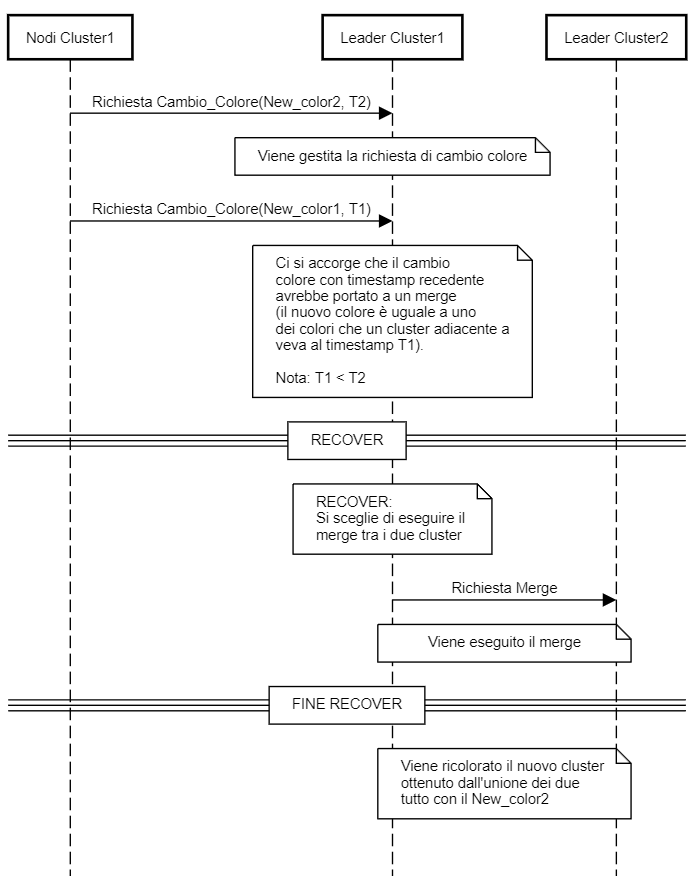
\includegraphics[width=0.8\textwidth,align=t]{images/concorrenza/caso1.png}
    \caption{Caso 1: Richiesta di cambio colore con timestamp anteriore che richiede un merge}
    \label{fig:caso1_concorrenza}
\end{figure}

\newpage
\paragraph{Caso 2: Richiesta di cambio colore con timestamp anteriore che non richiede un merge}\label{par:case2}

Nel caso in cui una richiesta con timestamp $T_1 < T_2$ non avrebbe comportato un merge al tempo $T_1$, ma l'operazione successiva con $T_2$ ha già effettuato un merge (Figura \ref{fig:caso2_concorrenza}):

\begin{itemize}
    \item La richiesta con timestamp $T_1$ viene ignorata, poiché lo stato corrente non rispecchia più le condizioni esistenti al tempo $T_1$.
\end{itemize}

Questo evita di sovrascrivere cambiamenti significativi con operazioni ormai obsolete.

\begin{figure}[H]
    \centering
    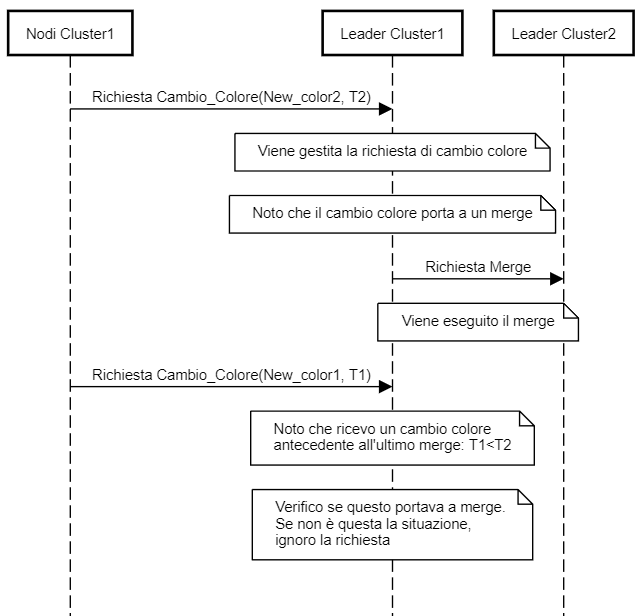
\includegraphics[width=0.8\textwidth,align=t]{images/concorrenza/caso2.png}
    \caption{Caso 2: Richiesta di cambio colore con timestamp anteriore che non richiede un merge}
    \label{fig:caso2_concorrenza}
\end{figure}

\newpage
\paragraph{Caso 3: Richiesta di merge ricevuta durante un cambio Colore con timestamp anteriore}\label{par:case3}

Quando un leader riceve una richiesta di merge mentre è in corso un'operazione di cambio colore con un timestamp anteriore (Figura \ref{fig:caso3_concorrenza}):

\begin{itemize}
    \item Il leader attende per un periodo di tempo prestabilito per consentire l'arrivo di eventuali richieste tardive.
    \item Se dopo il timeout non giungono ulteriori richieste, il leader procede con l'operazione di merge.
\end{itemize}

Questo meccanismo previene eventuali inconsistenze dovute all'ordine fuori sincronia delle operazioni.

\begin{figure}[H]
    \centering
    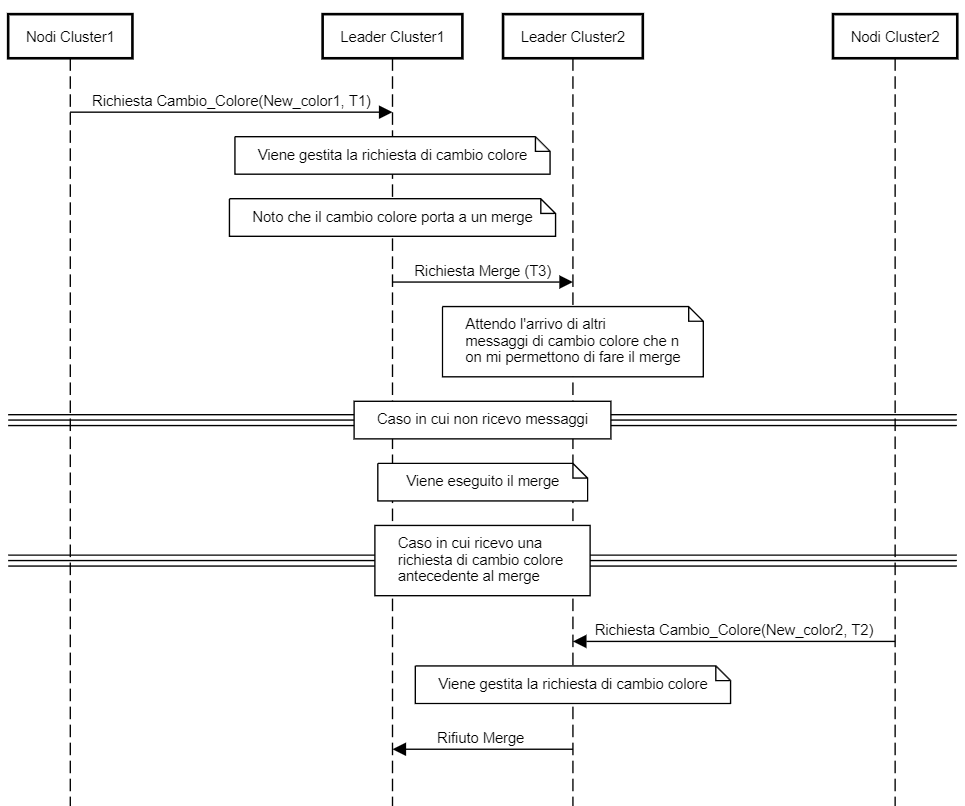
\includegraphics[width=1\textwidth,align=t]{images/concorrenza/caso3.png}
    \caption{Caso 3: Richiesta di merge ricevuta mentre è in corso un cambio colore con timestamp anteriore}
    \label{fig:caso3_concorrenza}
\end{figure}

\newpage
\paragraph{Caso ``Too Old'': gestione di una richiesta con timestamp troppo vecchio}\label{par:too_old}

Quando un leader riceve una richiesta di cambio colore o di merge con un timestamp troppo vecchio rispetto all'ultima operazione completata (Figura \ref{fig:caso_too_old}):

\begin{itemize}
    \item La richiesta viene ignorata (''droppata'') poiché il suo stato è ormai obsoleto rispetto alle operazioni più recenti.
\end{itemize}

Questo assicura che non vengano applicate modifiche non più pertinenti, evitando di introdurre inconsistenze nel sistema.

\begin{figure}[H]
    \centering
    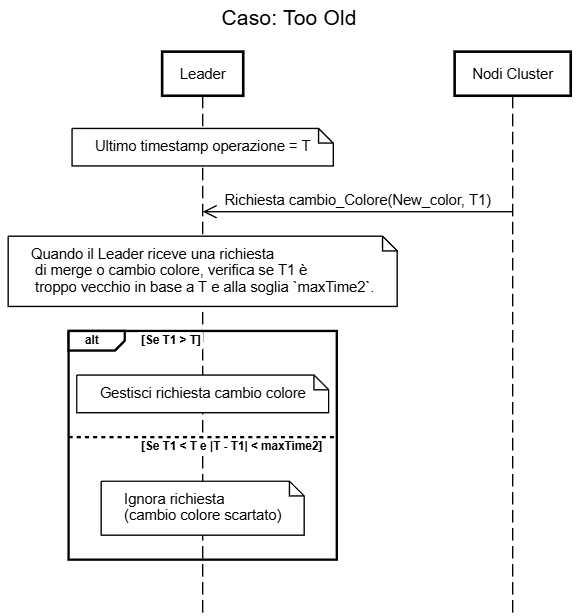
\includegraphics[width=0.70\textwidth,align=t]{images/concorrenza/too_old.png}
    \caption{Caso ``Too Old'': richiesta con timestamp troppo vecchio}
    \label{fig:caso_too_old}
\end{figure}

\newpage
\paragraph{Caso ``Cambio Colore durante Merge'': richiesta di cambio colore ricevuta durante un merge}\label{par:change_color_during_merge}

Se un leader riceve una richiesta di cambio colore o di merge mentre è in corso un'operazione di merge (Figura \ref{fig:change_color_during_merge}):

\begin{itemize}
    \item La richiesta viene accodata e verrà eseguita una volta completato il merge in corso.
\end{itemize}

In questo modo, si evita di alterare lo stato corrente mentre è in corso il merge, garantendo la coerenza e l'ordine delle operazioni.

\begin{figure}[H]
    \centering
    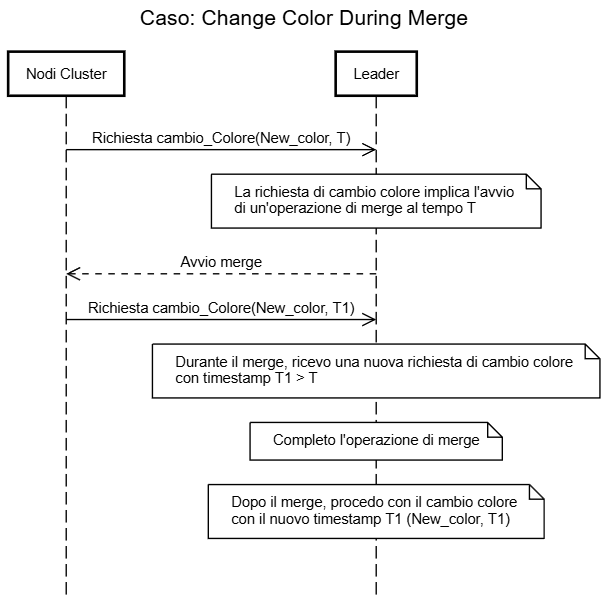
\includegraphics[width=0.75\textwidth,align=t]{images/concorrenza/change_color_during_merge.png}
    \caption{Caso ``Cambio Colore durante Merge'': richiesta di cambio colore durante un merge}
    \label{fig:change_color_during_merge}
\end{figure}

\newpage
\paragraph{Caso ``Doppio Merge'': merge tra cluster adiacenti con cambio colore}\label{par:double_merge}

Nel caso in cui due cluster adiacenti, inizialmente di colori diversi, ricevano una richiesta di cambio colore che li porta entrambi ad assumere lo stesso colore (Figura \ref{fig:double_merge}):

\begin{itemize}
    \item Si esegue un'operazione di merge, unendo i due cluster in un unico grande cluster con il nuovo colore comune.
\end{itemize}

Questo approccio garantisce che il sistema mantenga uno stato consistente e riduce la frammentazione dei cluster.

\begin{figure}[H]
    \centering
    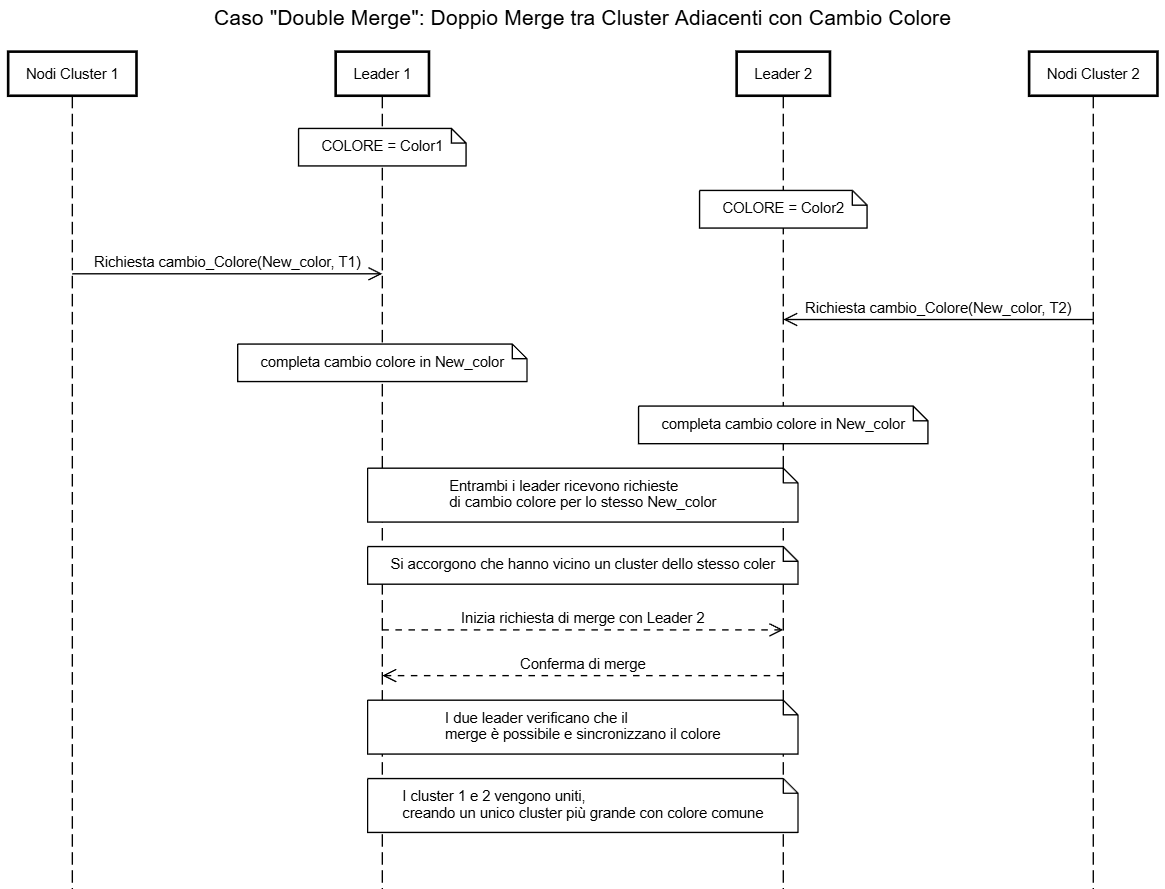
\includegraphics[width=1\textwidth,align=t]{images/concorrenza/doubleMerge.png}
    \caption{Caso ``Doppio Merge'': merge tra cluster adiacenti con cambio colore}
    \label{fig:double_merge}
\end{figure}

\subsection{Gestione dei fallimenti}\label{subsec:gestione_fallimenti}

La robustezza del sistema dipende dalla capacit\`a di gestire efficacemente i fallimenti dei nodi, sia leader che normali. Di seguito vengono dettagliate le strategie adottate per ricalcolare la struttura del cluster in caso di fallimenti, con particolare attenzione ai casi limite.

\subsubsection{1. Fallimento di un nodo leader}
\label{subsubsec:fallimento_leader}
Il leader di un cluster \`e fondamentale per la coordinazione e la comunicazione all'interno del cluster stesso. Tuttavia, il fallimento di un leader pu\`o generare scenari complessi, come la formazione di sotto-grafi disconnessi. Il sistema deve quindi gestire efficacemente tali situazioni per garantire la continuit\`a operativa e la coerenza del cluster.

\begin{itemize}
    \item \textbf{Monitoraggio tramite heartbeat}: i leader e il server scambiano continuamente messaggi di \texttt{heartbeat} per monitorare lo stato di salute dei leader.
    \item \textbf{Rilevamento del fallimento}: se il server o un altro leader non riceve un \texttt{heartbeat} da un leader entro un tempo prefissato (\textit{timeout}), assume che il leader sia fallito.
    \item \textbf{Gestione del partizionamento in sotto-grafi}:
    \begin{itemize}
        \item Quando un leader fallisce, il server elegge il nodo con l'\texttt{id} pi\`u basso rimasto e lo nomina come nuovo leader. 
        \item Il nuovo leader avvia una BFS per ristabilire la struttura gerarchica del suo sotto-grafo e comunica al server i nodi che fanno parte del sotto-grafo rimanente.
        \item Il server controlla se ci sono nodi non inclusi nel nuovo sotto-grafo e, per ogni gruppo di nodi sconnessi, elegge altri nuovi leader per gestire i restanti sotto-grafi.
        \item Il processo continua finché tutti i nodi disconnessi non vengono riassegnati a un leader e il cluster non \`e completamente ripristinato.
    \end{itemize}
    \item \textbf{Ricostruzione della struttura del cluster}:
    \begin{itemize}
        \item Durante la BFS, ogni nodo del sotto-grafo riassegnato aggiorna il proprio \texttt{leaderID} con quello del nuovo leader.
        \item Vengono sistemate le relazioni di \texttt{parent} e \texttt{child} tra i nodi per garantire la connessione all'interno del sotto-grafo.
        \item Vengono comunicati eventuali cluster adiacenti al nuovo leader in modo che possa aggiornare la rete overlay.
    \end{itemize}
\end{itemize}

\textbf{Casi limite da gestire}:

\begin{itemize}
    \item \textit{Partizionamento in pi\`u sotto-grafi disconnessi}: se il fallimento del leader causa la formazione di pi\`u sotto-grafi disconnessi, il server si assicura che ogni sotto-grafo venga gestito in modo indipendente con un nuovo leader. Il processo continua fino a quando tutti i nodi del cluster originario non sono stati riassegnati.
    \item \textit{Inconsistenze durante l'elezione}: per evitare condizioni di competizione (\textit{race conditions}), i nodi seguono una politica deterministica basata sull'\texttt{id} pi\`u basso per eleggere il nuovo leader in ciascun sotto-grafo.
\end{itemize}

\subsubsection{2. Fallimento di un nodo normale}
\label{subsubsec:fallimento_nodo_normale}
Il fallimento di un nodo non leader pu\`o avere impatti diversi sulla struttura del cluster, a seconda del ruolo del nodo e della sua posizione all'interno dell'albero di comunicazione.

\begin{itemize}
    \item \textbf{Nodo foglia}: se il nodo fallito \`e una foglia, il suo fallimento non interrompe la comunicazione tra gli altri nodi del cluster. Nessuna azione \`e necessaria.
    
    \item \textbf{Nodo interno}: se il nodo \`e interno e il suo fallimento interrompe la comunicazione tra parti del cluster, \`e necessario ricalcolare la struttura per ristabilire la connettivit\`a. Questo processo coinvolge diverse fasi dettagliate di seguito.

    \newpage
    \begin{enumerate}
        \item \textbf{Rilevamento del fallimento}:
        \begin{itemize}
            \item \textbf{Tentativi di comunicazione}: il nodo figlio del nodo fallito tenta di comunicare con il proprio \texttt{parent} per operazioni periodiche (ad esempio, messaggi di \texttt{heartbeat}) o in risposta a eventi specifici (come richieste di cambio colore).
            \item \textbf{Timeout e assunzione di fallimento}: se il nodo figlio non riceve risposta dopo un certo numero di tentativi, utilizzando meccanismi di \texttt{ack} (acknowledgment) e un intervallo di \textit{timeout}, assume che il \texttt{parent} sia fallito.
        \end{itemize}
        
        \item \textbf{Inizio della prima BFS (riconfigurazione)}:
        \begin{itemize}
            \item \textbf{Avvio di una BFS locale}: il nodo figlio avvia una \textit{Breadth-First Search} (BFS) per esplorare i nodi raggiungibili con lo stesso \texttt{leaderID}, inviando messaggi di \texttt{BFS\_Request} ai propri vicini. L'obiettivo \`e capire se esiste un percorso alternativo per raggiungere il leader originale.
            \item \textbf{Tracciamento delle richieste}: Durante la BFS, ogni nodo che riceve un \texttt{BFS\_Request} si segna da quale nodo \`e arrivata la richiesta, così da poter ripercorrere all'indietro il percorso seguito dalla richiesta una volta trovato un nodo connesso al leader.
        \end{itemize}
        
        \item \textbf{Analisi dei risultati della prima BFS}:
        \begin{enumerate}
            \item \textbf{Caso 1 - Cluster non isolato (leader raggiungibile)}: se la BFS raggiunge il leader originale il percorso seguito dalla prima BFS viene ripercorso all'indietro, aggiornando solo i nodi coinvolti direttamente nella ricostruzione del percorso e ristabilendo la connessione al nodo sconnesso aggiornando i \texttt{parent} dei nodi.

            \item \textbf{Caso 2 - Cluster isolato (leader non raggiungibile)}: se la BFS non trova alcun percorso per raggiungere il leader originale, significa che il sotto-grafo \`e diventato isolato dal cluster principale. Il nodo che ha avviato la BFS attende prima di avviare altre azioni:
            \begin{itemize}
                \item \textbf{Attesa delle risposte}: il nodo attende di ricevere risposte da tutti i nodi raggiunti dalla BFS. Se nessuno dei nodi risponde di essere collegato al leader, il nodo si autoproclama leader.
                \item \textbf{Avvio della seconda BFS (nuovo leader)}: una volta autoproclamato leader, il nodo avvia una seconda BFS per informare tutti i nodi del sotto-grafo che \`e diventato il nuovo leader.
                \item \textbf{Aggiornamento dei nodi}: tutti i nodi raggiunti dalla BFS aggiornano il proprio \texttt{leaderID} con quello del nuovo leader.
                \item \textbf{Comunicazione al server}: il nuovo leader invia un messaggio di \\ \texttt{NewLeaderAnnouncement} al server, informandolo della formazione del nuovo cluster e fornendo la lista dei nodi coinvolti.
            \end{itemize}
        \end{enumerate}
    \end{enumerate}
\end{itemize}

\subsection{Criteri di selezione del leader}

In un sistema distribuito come quello descritto, la selezione di un leader all'interno di un cluster di nodi \`e fondamentale per garantire efficienza operativa e tolleranza ai guasti. Nel contesto dell'algoritmo Flood-Fill distribuito, dove ogni nodo rappresenta un pixel, i leader devono essere scelti in modo da minimizzare la complessit\`a e garantire la robustezza. Di seguito, vengono discussi i criteri utilizzati per la selezione del leader.

\subsubsection{Attribuzione dell'ID ai nodi}

Ogni nodo nel sistema rappresenta un pixel di una matrice bidimensionale, e a ciascun nodo viene assegnato un identificatore unico (ID). Per generare l'ID dei nodi, si utilizzano le coordinate del pixel \texttt{(x, y)} all'interno della matrice. Esistono diversi metodi per attribuire un ID:

\begin{itemize}
    \item \textbf{Utilizzo delle coordinate \texttt{(x, y)}}: le coordinate stesse possono essere utilizzate come identificatore. In questo caso, l'ID del nodo sar\`a la coppia \texttt{(x, y)}, che rappresenta la posizione esatta del nodo nella matrice.
    
    \item \textbf{Linearizzazione delle coordinate}: per ottenere un ID scalare unico, \`e possibile convertire le coordinate \texttt{(x, y)} in un unico valore intero utilizzando la seguente formula:
    \[
    ID_{nodo} = y \times larghezza + x
    \]
    dove $larghezza$ \`e il numero di colonne della matrice. Questa rappresentazione permette di gestire pi\`u facilmente i nodi come valori interi unici.

    \item \textbf{Utilizzo dell'id del processo}: nello scenario di un sistema distribuito come questo, ogni nodo viene gestito come un processo a s\`e stante ed \`e possibile utilizzare l'id del processo come identificatore del nodo stesso.

\end{itemize}

Nel sistema proposto \`e stato scelto di utilizzare la terza soluzione, in quanto si adatta perfettamente al tipo di sistema. \'E stato inoltre scelto di sfruttare l'ideologia della prima proposta, creando dei riferimenti testuali \texttt{node\_X\_Y} per ogni PID\footnote{Process ID}, per facilitare il debugging degli scambi di messaggi e la lettura dei file di log e della struttura dati.

\subsubsection{Selezione del leader}

Una volta che a ciascun nodo \`e stato attribuito un ID, \`e necessario un criterio per la selezione del leader all'interno di ciascun cluster. I criteri di selezione possono variare in base alle esigenze del sistema, ma nel contesto di questo progetto si utilizza il seguente approccio:

\paragraph{ID pi\`u basso come leader}
Il criterio principale adottato \`e la selezione del nodo con l'ID pi\`u basso all'interno del cluster. Questo approccio offre diversi vantaggi:
\begin{itemize}
    \item \textbf{Semplicit\`a}: La selezione del leader basata sull'ID pi\`u basso \`e semplice da implementare e non richiede calcoli complessi o monitoraggi continui.
    \item \textbf{Determinismo}: Il nodo con l'ID pi\`u basso \`e sempre determinabile, garantendo che la selezione del leader sia univoca e ripetibile.
\end{itemize}

\paragraph{Failover e rielezione}
Nel caso in cui il leader selezionato fallisca, \`e previsto un meccanismo di failover automatico. I nodi del cluster avviano un'elezione per scegliere un nuovo leader, basata nuovamente sul criterio dell'ID pi\`u basso tra i nodi rimanenti. Questo processo garantisce che il cluster possa continuare a funzionare correttamente anche in presenza di guasti.

\newpage
\subsection{Vantaggi della soluzione proposta}

La soluzione scelta presenta diversi vantaggi:

\begin{itemize}
    \item \textbf{Scalabilit\`a}: trattando i cluster come nodi in un grafo overlay, il sistema pu\`o gestire efficacemente reti di grandi dimensioni.
    \item \textbf{Consistenza globale}: l'uso del database condiviso garantisce la sincronizzazione delle operazioni e la consistenza dello stato globale.
    \item \textbf{Robustezza ai fallimenti}: i meccanismi di gestione dei fallimenti assicurano che il sistema possa recuperare rapidamente da guasti di nodi leader o interni.
    \item \textbf{Efficienza}: la comunicazione \`e ottimizzata utilizzando i nodi leader all'interno dei cluster e il grafo overlay tra i leader.
\end{itemize}

\section{Piano di sviluppo}

Il piano di sviluppo del sistema \`e organizzato in sei fasi principali, ciascuna mirata a implementare aspetti cruciali del sistema distribuito, iniziando dalle funzionalit\`a di base fino ad arrivare alla gestione di consistenza e fault tolerance. Di seguito, vengono dettagliate le fasi del progetto:

\subsection*{Fase 1: Implementazione della comunicazione base e setup}

La prima fase \`e focalizzata sull'implementazione della comunicazione essenziale tra i nodi e sulla corretta configurazione della rete. L'obiettivo \`e garantire che ogni nodo possa scambiare messaggi con i nodi vicini e che la fase di setup, inclusa l'assegnazione dei leader e la costruzione del grafo dei cluster, funzioni correttamente.

\subsection*{Fase 2: Implementazione dell'algoritmo di cambio colore}

Una volta che la comunicazione base \`e stabilita, viene implementato l'algoritmo di cambio colore. Questo algoritmo permetter\`a a un nodo di avviare l'operazione di ricolorazione che si propagher\`a ai nodi adiacenti dello stesso cluster, sotto il coordinamento del leader.

\subsection*{Fase 3: Implementazione dell'algoritmo di merge}

Nella terza fase, viene sviluppato l'algoritmo di merge, che gestisce la fusione di cluster adiacenti quando questi acquisiscono lo stesso colore. L'algoritmo deve garantire che i leader dei cluster coinvolti collaborino per eseguire l'unione in maniera efficiente e consistente.

\subsection*{Fase 4: Implementazione del server di gestione del tempo e server centrale}

In questa fase, viene implementato un server centrale che gestisce i timestamp e coordina le operazioni tra i cluster. Il server avr\`a il compito di mantenere una visione globale dello stato del sistema e garantire che gli eventi vengano ordinati correttamente nel tempo, migliorando così la coerenza globale.

\subsection*{Fase 5: Gestione della consistenza globale}

Una volta implementato il server centrale, viene sviluppato un sistema di gestione della consistenza globale. Questo sistema garantisce che le operazioni distribuite, come i cambi di colore e i merge, siano ordinate in maniera corretta, evitando conflitti e garantendo che tutti i nodi abbiano una visione coerente dello stato del sistema.

\subsection*{Fase 6: Gestione dei fallimenti}

Nell'ultima fase, vengono implementati i meccanismi per gestire i fallimenti dei nodi, sia normali che leader. Questo include la rilevazione dei fallimenti, l'elezione di nuovi leader in caso di guasti e la riconfigurazione del sistema per mantenere la continuit\`a operativa anche in presenza di nodi falliti. L'obiettivo \`e garantire che il sistema sia resiliente e possa continuare a funzionare correttamente anche in condizioni di fault.

\section{Conclusioni}

La soluzione proposta, basata sul trattamento dei cluster come nodi in un grafo overlay e sull'uso di un database condiviso per la sincronizzazione, offre un equilibrio tra efficienza, scalabilit\`a e robustezza. I meccanismi di gestione della consistenza e dei fallimenti garantiscono il corretto funzionamento del sistema in ambienti distribuiti e soggetti a guasti.

\newpage

\chapter{Implementazione}

\section{Linguaggi di programmazione utilizzati}

Per questo progetto distribuito sono stati utilizzati due linguaggi di programmazione principali: \textbf{Erlang} e \textbf{Python}. Ciascuno di essi è stato scelto per le sue caratteristiche specifiche, che permettono di risolvere efficacemente problemi di distribuzione e visualizzazione.

\subsection{Erlang}

\textbf{Erlang} è stato scelto per la logica distribuita e la gestione dei nodi nel sistema, grazie alla sua robustezza e al supporto nativo per la concorrenza e la tolleranza ai guasti. Erlang è particolarmente adatto per applicazioni distribuite e fault-tolerant, ed è ampiamente utilizzato in ambiti come le telecomunicazioni e i sistemi di backend ad alta disponibilità.

\begin{itemize}
    \item \textbf{Gestione dei processi}: in Erlang, ogni nodo e leader è gestito come un processo indipendente. Questo permette al sistema di scalare facilmente e di mantenere l'isolamento dei fallimenti tra i nodi.
    \item \textbf{Pattern matching e concorrenza}: Erlang utilizza il pattern matching per la gestione dei messaggi e le strutture dati, facilitando la scrittura di codice conciso e mantenibile. La concorrenza è una funzionalità nativa del linguaggio, che permette ai processi di comunicare tramite messaggi in maniera asincrona.
    \item \textbf{Semplicità e resilienza}: Erlang implementa una semplice struttura di error handling in cui, invece di cercare di prevenire ogni possibile errore, i processi possono fallire e riavviarsi autonomamente. Questo modello “let it crash” è efficace in sistemi distribuiti dove i singoli componenti devono rimanere resilienti.
\end{itemize}

Erlang è quindi stato impiegato per la creazione e gestione dei nodi, la comunicazione tra essi e per mantenere il server centrale che coordina i leader e gestisce la propagazione dei messaggi.

\subsection{Python}

\textbf{Python} è stato scelto per la visualizzazione dei dati e l’interfaccia utente. Con la libreria \texttt{Flask}, è stato possibile implementare un server web per mostrare la matrice dei nodi e permettere l'interazione dell'utente, mentre \texttt{Matplotlib} è stato utilizzato per la grafica della griglia.

\begin{itemize}
    \item \textbf{Visualizzazione e interfaccia web}: Python, con \texttt{Flask} e \texttt{Matplotlib}, permette di creare interfacce web e rappresentazioni grafiche dei nodi in modo rapido e flessibile.
    \item \textbf{Aggiornamenti in tempo reale}: il supporto di \texttt{Flask-SocketIO} consente la comunicazione in tempo reale tra il backend e l'interfaccia utente, permettendo di aggiornare la visualizzazione della griglia dei nodi ogni volta che avvengono modifiche nel sistema.
    \item \textbf{Facilità d'integrazione con Erlang}: Python comunica con Erlang tramite un server TCP implementato in Erlang stesso. Questo approccio rende semplice l'integrazione e il passaggio di messaggi per operazioni come il cambio di colore dei nodi.
\end{itemize}

Python è quindi stato utilizzato come componente di frontend, fornendo una rappresentazione visiva intuitiva e permettendo l'interazione con i nodi per modificarne lo stato in tempo reale.

\subsection{Benefici della combinazione di Erlang e Python}

La combinazione di Erlang e Python ha permesso di sfruttare il meglio di entrambi i linguaggi:
\begin{itemize}
    \item \textbf{Distribuzione e resilienza} con Erlang per la gestione dei nodi e della logica di sistema.
    \item \textbf{Visualizzazione intuitiva e interattiva} con Python per fornire un’interfaccia utente che permette di osservare lo stato del sistema e interagire con esso.
\end{itemize}

Questo approccio ha consentito di mantenere un sistema distribuito robusto e allo stesso tempo di offrire una visualizzazione efficace e flessibile.

\section{Comandi principali}

In questa sezione sono descritti i comandi principali per avviare e configurare il sistema distribuito Flood-Fill. È possibile eseguire il sistema utilizzando due o tre shell separate, a seconda delle esigenze:
- \textbf{Con due shell}: ideale per un uso manuale, dove una shell avvia il backend Erlang e l’altra avvia il server Flask per l’interfaccia web.
- \textbf{Con tre shell}: utile per test automatizzati, aggiungendo una shell dedicata agli script di testing, che inviano richieste al sistema per verificare la correttezza e la resilienza in tempo reale.

I comandi descritti possono essere eseguiti sia manualmente per monitorare il sistema in modo interattivo, sia con script automatici di testing per simulare carichi di lavoro o condizioni specifiche.

\subsection{Avvio del backend Erlang}
Questo comando compila e avvia il backend, configurando una griglia di nodi e assegnando una porta per la comunicazione. 

\begin{tcolorbox}[title=Comandi di avvio in Erlang]
\begin{verbatim}
./compile_and_run.sh <ROWS> <COLUMNS> <FROM_FILE>
\end{verbatim}
\end{tcolorbox}

\noindent Dove:
\begin{itemize}
\item \texttt{<ROWS> <COLUMNS>} sono le dimensioni della griglia (ad esempio, 7 7 per una griglia 7x7).
\item \texttt{<FROM\_FILE>} specifica se i colori dei nodi devono essere letti da un file (\texttt{True}) o generati casualmente (\texttt{False}).
\end{itemize}

\subsection{Avvio del server Flask}
Il server Flask fornisce l’interfaccia web, che permette agli utenti di interagire con la griglia e cambiare i colori dei nodi.

\begin{tcolorbox}[title=Comandi di avvio del server Flask]
\begin{verbatim}
python3 grid_visualizer.py --debug <DEBUG_MODE> --port <PORTA>
\end{verbatim}
\end{tcolorbox}

\noindent Dove:
\begin{itemize}
    \item \texttt{<DEBUG\_MODE>} è \texttt{True} per attivare la modalità di debug, utile durante la fase di sviluppo.
    \item \texttt{<PORTA>} è la porta fornita dal backend Erlang per la comunicazione.
\end{itemize}

\subsection{Generazione di colori e operazioni casuali}
Questo comando genera una griglia di nodi con colori casuali e una lista di operazioni di cambio colore preimpostate, che possono essere usate per simulare vari scenari di test.

\begin{tcolorbox}[title=Generazione di colori e operazioni casuali]
\begin{verbatim}
python3 generate_changes_rand.py --rows <ROWS> --columns <COLUMNS> 
                                 --operations  <NUMBER_OPERATIONS>
\end{verbatim}
\end{tcolorbox}

\noindent Dove:
\begin{itemize}
    \item \texttt{<NUMBER\_OPERATIONS>} è il numero di cambi di colore casuali da generare.
\end{itemize}

\subsection{Esecuzione di test automatici}
Lo script di test automatico invia una serie di richieste di cambio colore al backend per verificare che i cambiamenti siano correttamente propagati e gestiti dal sistema.

\begin{tcolorbox}[title=Esecuzione di test automatici]
\begin{verbatim}
python3 script.py
\end{verbatim}
\end{tcolorbox}

\noindent Questi test permettono di osservare il comportamento del sistema in condizioni di carico e di verificare la consistenza delle operazioni di cambio colore e la resilienza del sistema in caso di errori.

\subsection{Esecuzione in shell multiple}
Per eseguire il sistema con \textbf{due shell}, avvia il backend Erlang nella prima shell e il server Flask nella seconda. Questa configurazione è adatta per un uso manuale, poiché consente di monitorare i log e l’interfaccia web direttamente.

Per eseguire il sistema con \textbf{tre shell}, usa una terza shell per avviare script di test automatici. Questo approccio è utile per verificare la robustezza del sistema, poiché permette di generare condizioni di carico e testare la propagazione dei cambi di colore tra i nodi.

\section{Records}

Le principali strutture dati utilizzate sono rappresentate dai record `node` e `leader`, che organizzano le informazioni di ciascun nodo e dei leader dei cluster. Questi record sono definiti in \texttt{node.erl} e permettono di gestire la posizione, i vicini e l'ID del leader per ciascun nodo.

\subsection{\texttt{node.hrl}}

Il record \texttt{node} rappresenta ciascun nodo del sistema. Contiene campi per le coordinate, il nodo parent, i figli, e lo stato di visita.

\begin{tcolorbox}[title=Definizione del record \texttt{node}]
\begin{verbatim}
  -record(node, {pid, x, y, leaderID, neighbors = []}).
\end{verbatim}
\end{tcolorbox}

\begin{itemize}
    \item \textbf{pid}: identificatore del processo Erlang associato al nodo.
    \item \textbf{x, y}: coordinate del nodo nella griglia.
    \item \textbf{leaderID}: pid del leader del cluster a cui il nodo appartiene.
    \item \textbf{neighbors}: lista dei pid dei nodi fisicamente adiacenti.
\end{itemize}

\subsection{\texttt{leader.hrl}}

Il record \texttt{leader} rappresenta i leader dei cluster, gestendo l’aggregazione di nodi con lo stesso colore. Questo record incapsula il record nodo, facilitando il passaggio da nodo normale a leader e viceversa. Ogni leader contiene informazioni sia sul proprio cluster che di quelle dei cluster adiacenti.

\begin{tcolorbox}[title=Definizione del record \texttt{leader}]
\begin{verbatim}
  -record(leader, {
      node, color, last\_event, adj\_clusters = [], cluster\_nodes = []
    }).
\end{verbatim}
\end{tcolorbox}

\begin{itemize}
    \item \textbf{node}: struttura dati del nodo leader.
    \item \textbf{color}: colore del cluster.
    \item \textbf{last\_event}: informazioni sull'ultima operazione eseguita sul cluster.
    \item \textbf{adj\_clusters}: lista dei cluster adiacenti.
    \item \textbf{cluster\_nodes}: lista dei pid dei nodi appartenenti al cluster.
\end{itemize}

\subsection{\texttt{event.hrl}}

Il record \texttt{event} viene usato per date una struttura alle informazioni sulle operazioni che vengono eseguite sui cluster.

\begin{tcolorbox}[title=Definizione del record \texttt{event}]
\begin{verbatim}
  -record(event, {timestamp, id, type, color, from}).
\end{verbatim}
\end{tcolorbox}

\begin{itemize}
    \item \textbf{timestamp}: tempo al momento della creazione di una nuova richiesta (operazione di cambio colore o merge).
    \item \textbf{id}: identificatore univoco della richiesta. Essendo progressivi, nel caso di concorrenza (i.e. timestamp equivalente) viene usato per determinare l'ordine.
    \item \textbf{type}: tipo di operazione (\texttt{color} o \texttt{merge}).
    \item \textbf{color}: colore associato all'operazione.
    \item \textbf{from}: leaderID del cluster in cui avver\`a l'operazione. Usato dal server per conoscere il richiedente dell'operazione.
\end{itemize}

\section{Moduli}

\subsection{\texttt{node.erl}}

Il modulo \texttt{node.erl} è progettato per gestire la creazione, la gestione e la comunicazione tra i nodi in una rete distribuita. Esso permette di coordinare dinamicamente le operazioni sui nodi e sui leader all'interno del sistema, gestendo anche eventi come cambi di colore, elezione di nuovi leader e fusioni di cluster.

Il modulo contiene le seguenti funzioni principali:

\begin{itemize}
    \item \texttt{new\_node/8}: questa funzione crea un nuovo nodo con parametri specifici come la posizione, il leader, i vicini e altre proprietà essenziali. Ogni nodo è dotato di un identificativo unico (PID) e può interagire con i vicini e il leader assegnato.

    \item \texttt{new\_leader/5}: crea e configura un nodo come leader. Un leader coordina i nodi all'interno di un cluster, assegnandosi il proprio PID come leader ID. La funzione inizializza inoltre attributi specifici come il colore del cluster e le informazioni sui cluster adiacenti.

    \item \texttt{create\_node/2}: avvia il processo per un nodo leader, aggiornando il suo PID e garantendo che possa comunicare con gli altri nodi della rete. Questa funzione spawna un processo per il ciclo di vita del nodo, rendendolo operativo.

    \item \texttt{leader\_loop/1}: \`e il ciclo principale del leader. Questa funzione permette al leader di ricevere e gestire continuamente i messaggi, garantendo una risposta reattiva agli eventi che si verificano nella rete, come aggiornamenti di cluster o cambiamenti di colore.

    \item \texttt{node\_loop/1}: ciclo principale per i nodi standard, che processa i messaggi ricevuti e permette al nodo di rispondere a richieste di cambio colore, aggiornamenti di leader e altre interazioni con i nodi vicini.

\end{itemize}

\noindent
Lo scopo del modulo \texttt{node.erl} è fornire una struttura robusta per la gestione di una rete distribuita di nodi, dove ciascun nodo può essere configurato come nodo standard o leader. La flessibilità del modulo consente di implementare dinamicamente una rete in cui i nodi possono cambiare colore, coordinarsi con i leader e gestire le proprie interazioni in modo distribuito. Questo modulo abilita la gestione dinamica dei cluster e la resilienza a eventuali errori o modifiche, come l'elezione di nuovi leader e la fusione di cluster adiacenti. In questo modo, è possibile mantenere la consistenza dei colori e la corretta organizzazione dei nodi anche in scenari complessi.

\subsection{\texttt{event.erl}}

Il modulo \texttt{event.erl} gestisce la creazione, la gestione e il confronto degli eventi in un sistema distribuito. Gli eventi rappresentano azioni o cambiamenti di stato e sono utilizzati per mantenere la consistenza tra i componenti distribuiti. Ogni evento include informazioni come il timestamp, un ID unico, il tipo di evento, il colore associato e il PID del leader che ha generato l'evento.

Le principali responsabilità del modulo includono:

\begin{itemize}
    \item \textbf{Creazione degli eventi}: il modulo fornisce funzioni per creare eventi con un timestamp attuale o con un timestamp specificato, utile per scenari di testing o ricostruzione di eventi storici.

    \item \textbf{Confronto degli eventi}: implementa una funzione per confrontare due eventi, consentendo al sistema di stabilire l'ordine temporale degli eventi in base al timestamp e, in caso di parità, all'ID unico di ciascun evento.

\end{itemize}

\noindent
Le principali funzioni del modulo sono le seguenti:

\begin{itemize}
    \item \texttt{new/3}: crea un nuovo evento con il timestamp attuale. Gli attributi dell'evento includono il tipo, il colore e il leader che ha originato l'evento. Questa funzione è utilizzata per la generazione di eventi in tempo reale.

    \item \texttt{new\_with\_timestamp/4}: consente la creazione di un evento con un timestamp specificato, utile in contesti di testing o per ricostruire eventi passati. L'evento conserva le stesse proprietà di \texttt{new/3}, ma accetta un timestamp definito dall'utente.

    \item \texttt{greater/2}: confronta due eventi per stabilire il loro ordine temporale. Se il primo evento ha un timestamp più recente del secondo, viene considerato ``maggiore''. In caso di parità di timestamp, l'ID unico dell'evento è usato per determinare l'ordine. Questa funzione è essenziale per gestire correttamente la sequenza degli eventi nel sistema distribuito.

\end{itemize}

\noindent
Il modulo \texttt{event.erl} è fondamentale per garantire una gestione ordinata e coerente degli eventi all'interno del sistema distribuito, assicurando che le azioni vengano processate nel corretto ordine temporale, anche in situazioni di conflitto. Utilizzando i timestamp e gli ID unici, il modulo permette al sistema di risolvere i conflitti e mantenere una visione sincronizzata dello stato distribuito.

\subsection{\texttt{operation.erl}}

Il modulo \texttt{operation.erl} fornisce una serie di funzioni per la gestione di operazioni distribuite in un sistema di cluster, con particolare attenzione alla gestione dei colori dei cluster, alla fusione di cluster adiacenti e alle operazioni di recupero in caso di guasto di un leader. Questo modulo garantisce che i nodi nei cluster mantengano una colorazione coerente e che ogni cluster abbia un leader attivo.

Le principali funzionalità del modulo sono:

\begin{itemize}
    \item \textbf{Gestione dei cambi di colore}: funzioni come \texttt{change\_color/2} e \texttt{do\_change\_color/2} permettono di aggiornare il colore di un leader e di propagare questa informazione ai cluster adiacenti, mantenendo la consistenza dei colori. Questo è utile per evitare conflitti tra i cluster.

    \item \textbf{Utilità per la fusione dei cluster}: funzioni come \texttt{merge\_adjacent\_clusters/4} e \texttt{wait\_for\_merge\_response/4} gestiscono la fusione di cluster adiacenti quando questi condividono lo stesso colore. Queste funzioni aggiornano correttamente la lista dei nodi e dei cluster adiacenti.

    \item \textbf{Operazioni di recupero}: la funzione \texttt{promote\_to\_leader/5} permette di promuovere un nodo a leader, utile per il recupero da guasti dei leader. In questo modo, ogni cluster ha un leader attivo, garantendo la continuità operativa e la comunicazione con i cluster adiacenti.

\end{itemize}

\noindent
Le principali funzioni del modulo sono le seguenti:

\begin{itemize}
    \item \texttt{change\_color/2}: inizia il cambiamento di colore di un leader e propaga questo aggiornamento ai cluster adiacenti, notificando anche il server. La funzione si assicura che i cambiamenti siano visibili in tutta la rete.

    \item \texttt{merge\_adjacent\_clusters/4}: gestisce il processo di fusione tra un leader e cluster adiacenti con lo stesso colore. Assicura che i nodi e le liste di adiacenza siano aggiornati durante le operazioni di fusione.

    \item \texttt{remove\_cluster\_from\_adjacent/2}: rimuove un cluster specifico dalla lista dei cluster adiacenti, utile in caso di guasto del leader.

    \item \texttt{promote\_to\_leader/5}: promuove un nodo a leader, inizializzando le sue informazioni di cluster e di adiacenza. È una funzione di recupero fondamentale per garantire che i cluster rimangano operativi anche in caso di guasti.

    \item \texttt{send\_periodic\_updates/1} e \texttt{broadcast\_leader\_update/1}: invia periodicamente aggiornamenti sul colore e sul leader corrente a tutti i nodi del cluster e ai cluster adiacenti, garantendo una sincronizzazione continua delle informazioni.

\end{itemize}

\noindent
Il modulo \texttt{operation.erl} è essenziale per il mantenimento dell'integrità e della coerenza di un sistema distribuito basato su cluster, gestendo in modo dinamico i colori dei cluster, la fusione tra cluster adiacenti e il recupero da guasti dei leader. Grazie alle sue funzioni, il sistema può adattarsi ai cambiamenti e mantenere una rete di comunicazione affidabile tra i cluster.

\subsection{\texttt{server.erl}}

Il modulo \texttt{server.erl} implementa il processo server per la gestione e il coordinamento di un sistema distribuito di nodi e cluster. Le principali responsabilità del server includono l'inizializzazione dei nodi, il monitoraggio dei leader, la gestione della consistenza dei colori dei cluster e il salvataggio dello stato del sistema in formato JSON per scopi di persistenza.

\paragraph{Funzionalità principali:}
\begin{itemize}
    \item \textbf{Setup dei nodi}: gestisce l'inizializzazione dei nodi tramite richieste di setup, assegnando leader e aggiornando lo stato del sistema.
    \item \textbf{Monitoraggio dei leader e failover}: monitora i leader, promuovendo nuovi leader in caso di guasti, per garantire la continuità.
    \item \textbf{Consistenza del colore dei cluster}: verifica che i cluster adiacenti abbiano colori unici e richiede cambi di colore se necessario.
    \item \textbf{Persistenza dei dati}: salva periodicamente lo stato del server, inclusa la configurazione di nodi e leader, in file JSON per consentire il recupero dello stato del sistema.
\end{itemize}

\paragraph{Funzioni principali:}
\begin{itemize}
    \item \texttt{start\_server/1}: avvia il processo server, inizializzandolo con strutture dati vuote per tracciare i nodi e i leader.
    \item \texttt{server\_loop/4}: \`e il ciclo principale che gestisce i messaggi di setup, aggiornamenti dei leader, richieste di cambio colore e aggiornamenti di adiacenza.
    \item \texttt{start\_phase2\_for\_all\_leaders/5}: avvia la \textit{Fase 2} per tutti i leader, raccogliendo informazioni di adiacenza e salvando la configurazione finale.
    \item \texttt{collect\_leader\_responses/3}: raccoglie le risposte dei leader entro un timeout, confermando la loro attività nel sistema.
    \item \texttt{finish\_setup/4}: conclude la fase di setup, istruendo ciascun leader a salvare la propria configurazione localmente.
    \item \texttt{save\_leader\_configuration\_json/1}: converte le configurazioni dei leader in formato JSON e le salva in un file per la persistenza.
    \item \texttt{notify\_adjacent\_clusters\_to\_remove\_cluster/2} e \\ \texttt{notify\_adjacent\_clusters\_about\_new\_leader/3}: aggiornano i cluster adiacenti per rimuovere riferimenti a un leader terminato o aggiornare riferimenti a un leader appena promosso.
\end{itemize}

\noindent
Il modulo \texttt{server.erl} è fondamentale per gestire la configurazione iniziale del sistema, monitorare i leader per prevenire guasti e assicurare che ogni cluster mantenga un colore univoco rispetto ai cluster adiacenti. Le funzioni di salvataggio in JSON permettono di mantenere uno snapshot dello stato corrente del sistema, rendendolo pronto per il debug e il recupero.

\subsection{\texttt{setup.erl}}

Il modulo \texttt{setup.erl} implementa la fase di configurazione per un sistema distribuito di nodi. Ogni nodo partecipa a un processo di configurazione per stabilire la connettività con i vicini, propagare le informazioni di leader e colore e identificare i cluster adiacenti all'interno della rete.

\paragraph{Funzionalità principali:}
\begin{itemize}
    \item \textbf{Gestione della connessione dei nodi}: ogni nodo stabilisce la propria connessione con i vicini, aggiornando le informazioni sul leader e la struttura del cluster.
    \item \textbf{Propagazione delle informazioni di configurazione}: durante la propagazione, i nodi scambiano informazioni di configurazione per stabilire la gerarchia e la struttura dei leader.
    \item \textbf{Identificazione dei cluster adiacenti}: i nodi costruiscono una lista dei cluster vicini richiedendo informazioni sul leader ai nodi connessi.
    \item \textbf{Raccolta dei nodi adiacenti}: i nodi raccolgono informazioni dai vicini per stabilire una lista completa dei nodi direttamente connessi.
\end{itemize}

\paragraph{Funzioni principali:}
\begin{itemize}
    \item \texttt{setup\_loop/3}: loop principale per gestire le richieste di configurazione iniziali, propagare informazioni e aggiornare lo stato di connettività.
    \item \texttt{setup\_loop\_propagate/7}: gestisce la propagazione della configurazione, inviando richieste di configurazione ai vicini e raccogliendo gli ack.
    \item \texttt{wait\_for\_ack\_from\_neighbors/7}: attende in modo ricorsivo le risposte dai vicini, aggiornando lo stato in base ai messaggi ricevuti.
    \item \texttt{gather\_adjacent\_clusters/5}: identifica i cluster adiacenti richiedendo le informazioni sul leader ai nodi vicini.
    \item \texttt{gather\_adjacent\_nodes/3}: raccoglie i nodi direttamente connessi costruendo una lista completa dei vicini.
\end{itemize}

\noindent
Il modulo \texttt{setup.erl} è progettato per essere utilizzato in ambienti distribuiti, dove ogni nodo opera in modo indipendente ma deve collaborare con altri per formare cluster, assegnare leader e propagare i dati di connettività. La gestione dei timeout consente al modulo di rispondere a nodi non disponibili, garantendo robustezza durante la configurazione iniziale. Questo modulo si affida a funzioni di utilità come \texttt{utils:save\_data/1} per gestire compiti comuni e per migliorare l'efficienza.

\subsection{\texttt{start\_system.erl}}

Il modulo \texttt{start\_system.erl} gestisce l'inizializzazione e la configurazione di un sistema distribuito di nodi in una griglia $N \times M$. Fornisce funzionalità per creare un server, generare nodi con attributi di colore, assegnare i vicini e sincronizzare la configurazione iniziale assicurando che i nodi ricevano e confermino la configurazione.

\paragraph{Caratteristiche principali:}
\begin{itemize}
    \item \textbf{Inizializzazione della griglia}: configura i nodi in una griglia $N \times M$.
    \item \textbf{Assegnazione dei colori}: ogni nodo riceve un colore unico, caricato da un file o selezionato da una palette predefinita.
    \item \textbf{Assegnazione dei vicini}: configura le relazioni di vicinato per ciascun nodo in base alla posizione nella griglia.
    \item \textbf{Sincronizzazione della configurazione}: attende l'acknowledgment di tutti i nodi prima di iniziare la configurazione del server.
    \item \textbf{Salvataggio della configurazione finale}: salva i dati di configurazione dei nodi in formato JSON.
\end{itemize}

\paragraph{Funzioni principali:}
\begin{itemize}
    \item \texttt{start/3}: inizializza il server e genera una griglia $N \times M$ di nodi, assegnando colori e vicini. Attende l'acknowledgment di ogni nodo prima di iniziare il setup del server.
    \item \texttt{load\_colors\_from\_file/1}: carica i colori da un file, convertendo ciascuna riga in un atomo.
    \item \texttt{save\_nodes\_data/1}: converte i dati dei nodi in formato JSON e li salva in un file.
    \item \texttt{node\_to\_json/11}: converte i campi di un nodo in una stringa JSON formattata.
    \item \texttt{find\_neighbors/4}: identifica i nodi vicini per un nodo specifico nella griglia $N \times M$ in base alle coordinate.
\end{itemize}

\paragraph{Precondizioni e postcondizioni:}
\begin{itemize}
    \item \textbf{Precondizioni}: devono essere specificate le dimensioni della griglia (N, M). Se \texttt{FromFile} è impostato su \texttt{true}, deve essere presente un file valido con i colori.
    \item \textbf{Postcondizioni}: un processo server viene creato e tutti i nodi sono inizializzati con i loro colori e vicini. I dati finali della configurazione dei nodi vengono salvati in un file JSON per uso futuro.
\end{itemize}

\noindent
Il modulo \texttt{start\_system.erl} è utilizzato come punto d'ingresso per configurare il sistema, incluso server, nodi e vicini, e viene invocato con le dimensioni desiderate della griglia. Questo modulo supporta sia la configurazione tramite un file di colori che tramite una palette predefinita, rendendolo flessibile per vari scenari di inizializzazione.

\subsection{\texttt{tcp\_server.erl}}

Il modulo \texttt{tcp\_server.erl} implementa un server TCP che riceve comandi dai client per controllare un sistema distribuito di nodi. Consente la gestione di comandi come il cambio di colore di un nodo o la terminazione di un nodo specifico, elaborando e inoltrando i messaggi al processo corrispondente.

\paragraph{Caratteristiche principali:}
\begin{itemize}
    \item \textbf{Server TCP}: avvia un server TCP e ascolta su una porta disponibile.
    \item \textbf{Gestione comandi}: riceve comandi dai client, come il cambio colore o la terminazione di nodi, e li elabora.
    \item \textbf{Validazione input}: valida e converte i parametri dei messaggi ricevuti, come PID e colori.
    \item \textbf{Interazione in tempo reale}: consente un controllo dinamico dei nodi tramite input dei client.
\end{itemize}

\paragraph{Funzioni principali:}
\begin{itemize}
    \item \texttt{start/0}: avvia il server TCP, apre una porta per ascoltare le connessioni e gestisce i client in modo concorrente.
    \item \texttt{listen/1}: ascolta le connessioni TCP in arrivo e crea un processo separato per ogni client.
    \item \texttt{loop/1}: gestisce il ciclo principale di ricezione dei messaggi da un client e l'inoltro della risposta.
    \item \texttt{handle\_message/2}: elabora un messaggio client, distinguendo comandi come il cambio di colore o la terminazione.
    \item \texttt{convert\_to\_pid/1}: converte una stringa in un PID Erlang, se valido.
    \item \texttt{convert\_to\_color/1}: converte una stringa in un colore della palette predefinita.
    \item \texttt{parse\_time/3}: converte stringhe di ore, minuti e secondi in una tupla temporale.
\end{itemize}

\noindent
Il modulo \texttt{tcp\_server.erl} fornisce un'interfaccia per la gestione dinamica del sistema distribuito, consentendo modifiche in tempo reale ai nodi attraverso comandi client. È ideale per ambienti in cui è necessario interagire e monitorare un sistema distribuito di nodi con feedback immediato.

\subsection{\texttt{utils.erl}}

Il modulo \texttt{utils.erl} contiene funzioni di utilità per la gestione e l'elaborazione dei dati in un sistema distribuito di nodi e cluster. Esso include operazioni su liste, formattazione, manipolazione di dati JSON, log degli eventi, e backup dei dati, promuovendo modularità e riutilizzabilità.

\paragraph{Caratteristiche principali:}
\begin{itemize}
    \item \textbf{Operazioni su liste}: funzioni per rimuovere duplicati, unire liste, filtrare elementi e verificare condizioni specifiche su elenchi di nodi o cluster.
    \item \textbf{Formattazione}: funzioni di conversione e formattazione per rappresentare colori, PID e timestamp in formati specifici.
    \item \textbf{Gestione JSON}: funzioni per convertire strutture dati in JSON e salvarle su file per persistenza.
    \item \textbf{Logging}: registrazione di operazioni di sistema con timestamp per facilitare il debug e la tracciabilità.
    \item \textbf{Backup dati}: funzioni per salvare i dati di nodi e leader su file, supportando il ripristino e la revisione.
\end{itemize}

\paragraph{Funzioni principali:}
\begin{itemize}
    \item \texttt{remove\_duplicates/1}: rimuove elementi duplicati da una lista.
    \item \texttt{unique\_leader\_clusters/1}: raccoglie cluster unici in base a LeaderID.
    \item \texttt{check\_same\_color/2}: verifica se un cluster adiacente ha lo stesso colore.
    \item \texttt{normalize\_color/1}: converte un colore in un atomo se necessario.
    \item \texttt{pid\_to\_string/1}: converte un PID in una stringa compatibile con JSON.
    \item \texttt{log\_operation/1}: registra un'operazione con un timestamp in un file di log.
    \item \texttt{save\_leader\_data\_to\_file/1}: salva i dati del leader in formato JSON.
    \item \texttt{save\_node\_data\_to\_file/1}: salva i dati del nodo in formato JSON.
\end{itemize}

\noindent
Il modulo \texttt{utils.erl} fornisce strumenti essenziali per la gestione e il controllo del sistema, semplificando le operazioni comuni e garantendo la consistenza dei dati nei nodi e cluster distribuiti. È fondamentale per la manutenzione e la scalabilità del sistema.

\section{Scripts}\label{sec:scripts}

\subsection{\texttt{grid\_visualizer.py}}

Lo script Python \texttt{grid\_visualizer.py} implementa una visualizzazione grafica in tempo reale per una griglia di nodi e cluster di un sistema distribuito. Sviluppato con Flask per il server web e Matplotlib per la generazione della griglia, lo script permette agli utenti di osservare e gestire lo stato dei nodi direttamente dal browser. Grazie all'uso di Flask-SocketIO, supporta aggiornamenti in tempo reale tramite WebSocket.

\paragraph{Funzionalità principali:}
\begin{itemize}
    \item \textbf{Visualizzazione della griglia}: la griglia mostra i nodi, ciascuno colorato in base al leader di appartenenza, e connessioni visive tra i nodi dello stesso cluster, evidenziando i leader con un'etichetta speciale ``L''.
    \item \textbf{Gestione dei colori in tempo reale}: gli utenti possono modificare i colori dei nodi direttamente dall'interfaccia web. Le richieste di cambio colore vengono inoltrate al server Erlang, che aggiorna i nodi nel sistema distribuito.
    \item \textbf{Aggiornamenti automatici e logging}: la visualizzazione della griglia si aggiorna ogni 30 secondi o al rilevamento di modifiche nei dati, notificando i client via WebSocket. Ogni modifica viene registrata in un file Jupyter Notebook (\texttt{history\_log.ipynb}) e salvata come snapshot.
\end{itemize}

\paragraph{Struttura del codice:}
\begin{itemize}
    \item \texttt{load\_leaders\_data()}: carica i dati dei leader dai file JSON, cruciali per colorare i nodi e definire i cluster.
    \item \texttt{draw\_matrix()}: genera la rappresentazione grafica della griglia, evidenziando leader e connessioni tra i nodi.
    \item \texttt{clear\_notebook() e log\_change\_notebook()}: gestiscono il logging delle modifiche, svuotando il notebook al riavvio e registrando le variazioni nel tempo.
    \item \texttt{send\_color\_change\_request()}: invio di richieste di cambio colore al server Erlang tramite TCP.
    \item \texttt{clear\_snapshots\_folder()}: pulisce la cartella snapshot all’avvio per evitare sovrapposizioni di immagini.
\end{itemize}

\paragraph{Utilizzo:}
\begin{itemize}
    \item Avviare lo script con il comando:

      \hspace{20pt}\texttt{python grid\_visualizer.py --port <PORT> --debug <DEBUG\_MODE>}.
    \item I parametri configurabili includono: 
    \begin{itemize}
        \item \texttt{port}: la porta TCP per comunicare con Erlang.
        \item \texttt{debug}: attiva/disattiva la modalità di debug.
        \item \texttt{leaders\_file}, \texttt{nodes\_file}, \texttt{img\_path}, \texttt{notebook\_path}, \texttt{snapshots\_folder}: percorsi per i file JSON dei leader e dei nodi, immagine della matrice, file notebook di log, e la cartella di snapshot.
    \end{itemize}
\end{itemize}

\subsection{\texttt{generate\_changes\_rand.py}}\label{sec:random_changes}

Il file \texttt{generate\_changes\_rand.py} è un utile script Python progettato per gestire un sistema distribuito di nodi, permettendo di modificare colori e gestire processi in modo programmato e casuale. Lo script interagisce con un server Erlang tramite connessioni TCP, inviando comandi per modificare i colori dei nodi o terminare processi, facilitando così la gestione e il testing di configurazioni di cluster distribuiti.

\paragraph{Funzionalità Principali:}
\begin{itemize}
    \item \textbf{Reset del database}: cancella tutte le sottodirectory presenti nella cartella principale \texttt{DB} per azzerare i dati dei nodi.
    \item \textbf{Generazione file di colori}: crea un file di testo (\texttt{colors.txt}) contenente assegnazioni di colori per una griglia di nodi specificata.
    \item \textbf{Richieste di cambio colore}: invia comandi per cambiare i colori dei nodi al server Erlang tramite socket TCP.
    \item \textbf{Terminazione processi}: identifica e termina processi in esecuzione su una specifica porta per facilitare la gestione e il setup del server.
    \item \textbf{Operazioni multiple}: esegue operazioni multiple di cambio colore e termina processi in modo casuale in base a parametri di input.
\end{itemize}

\paragraph{Struttura del codice:}
\begin{itemize}
    \item \texttt{elimina\_DB()}: cancella tutte le directory nella cartella \texttt{DB} per un reset completo.
    \item \texttt{generate\_colors\_file()}: genera un file \texttt{colors.txt} con i colori per ogni nodo della griglia, in base alle dimensioni specificate.
    \item \texttt{send\_color\_change\_request()}: invia una richiesta al server Erlang per cambiare il colore di un nodo specifico.
    \item \texttt{perform\_multiple\_operations()}: esegue un numero definito di operazioni (cambi di colore) casuali sui nodi.
\end{itemize}

\paragraph{Utilizzo:}
\begin{itemize}
    \item Eseguire lo script con i seguenti argomenti opzionali:
        \begin{itemize}
            \item \texttt{rows}: numero di righe della matrice di nodi ($N$).
            \item \texttt{columns}: numero di colonne della matrice di nodi ($M$).
            \item \texttt{operations}: numero di operazioni di cambio colore da effettuare.
        \end{itemize}
    \item Esempio di utilizzo:
      
      \hspace{20pt}\texttt{python generate\_changes\_rand.py \-\-rows 5 \-\-columns 5 \-\-operations 10}
\end{itemize}

\subsection{\texttt{script.py}}\label{sec:script}

Il file \texttt{script.py} è un script Python utilizzato per gestire e testare una griglia di nodi in un sistema distribuito. Lo script è particolarmente utile per verificare la reattività e la coerenza del sistema durante operazioni di cambio colore e condizioni di merge. Comunica con un server Erlang tramite TCP, consentendo di inviare richieste di cambio colore ai nodi e di eseguire scenari di test specifici per analizzare la stabilità del sistema in caso di aggiornamenti simultanei o condizioni temporali complesse.

\paragraph{Funzionalit\`a principali:}
\begin{itemize}
    \item \textbf{Reset del database}: la funzione \texttt{elimina\_DB} rimuove tutte le sottodirectory nella cartella \texttt{DB}, azzerando lo stato dei nodi per avviare un nuovo test.
    \item \textbf{Configurazione dei colori}: la funzione \texttt{generate\_colors\_file} genera un file \\
    \texttt{colors.txt} con i colori di ciascun nodo in una griglia $N \times M$. I colori possono essere generati casualmente o secondo una tavolozza predefinita.
\end{itemize}

\paragraph{Struttura del codice:}
\begin{itemize}
    \item \texttt{elimina\_DB()}: cancella tutte le sottodirectory in \texttt{DB}, ripristinando lo stato iniziale del sistema.
    \item \texttt{generate\_colors\_file(N, M, random\_colors)}: genera un file di colori per una griglia $N \times M$, utilizzando colori casuali o una tavolozza predefinita.
    \item \texttt{send\_color\_change\_request(pid, color, timestamp, PORT)}: invia una richiesta \\TCP al server Erlang per cambiare il colore di un nodo specifico.
    \item \texttt{get\_pid\_by\_coordinates(data, x, y)}: trova l’identificatore del nodo basandosi sulle coordinate specificate.
    \item \texttt{case1, case2, case3, too\_old, change\_color\_during\_merge, doubleMerge}: Ciascuna di queste funzioni rappresenta un caso di test diverso che simula gli scenari presentati in \ref{subsec:gestione_consistenza}. Ciascun test e la sua struttura viene spiegato nella repository del progetto.
\end{itemize}


\paragraph{Utilizzo:}
Per utilizzare lo script, è possibile eseguirlo e seguire le istruzioni a schermo per specificare dimensioni della matrice, resettare il database e configurare la porta del server.
Una volta configurato, l’utente può scegliere tra i vari casi di test da eseguire.

Esempio di utilizzo:
\begin{verbatim}
    python3 script.py
\end{verbatim}


\paragraph{Nota:}
Ogni test fornisce uno scenario unico per valutare la robustezza del sistema distribuito, testando la sensibilità ai tempi di aggiornamento, la coerenza durante le operazioni simultanee e la capacità di rispondere a merge di cluster.

\section{File di backup e logging}

Nel sistema distribuito progettato, vengono generati diversi file per memorizzare localmente i dati di ciascun nodo e tracciare le operazioni eseguite. Di seguito è riportata una descrizione dettagliata di ciascun file.

\paragraph{\texttt{data/nodes\_data.json}} Questo file contiene le informazioni dei nodi creati durante l'inizializzazione del sistema. Ogni nodo è rappresentato in una struttura JSON che include:
\begin{itemize}
    \item \texttt{pid}: ID del processo Erlang che rappresenta il nodo.
    \item \texttt{x}: coordinata orizzontale del nodo nella griglia.
    \item \texttt{y}: coordinata verticale del nodo nella griglia.
\end{itemize}
Questo file è utile per tenere traccia della disposizione dei nodi e delle loro caratteristiche di base.

\paragraph{\texttt{data/leaders\_data.json}} Questo file memorizza i dati di ciascun leader, incluse le informazioni sui cluster associati. Ogni leader è rappresentato da una struttura JSON che include:
\begin{itemize}
    \item \texttt{color}: il colore assegnato al leader, che identifica il cluster.
    \item \texttt{adjacent\_clusters}: una lista di cluster adiacenti rappresentata da strutture \texttt{\{pid, color, leader\_id\}}, dove \texttt{leader\_id} è l'ID del leader del cluster adiacente, \texttt{pid} rappresenta un nodo vicino, e \texttt{color} è il colore associato a quel cluster.
    \item \texttt{nodes}: una lista degli ID di processo dei nodi appartenenti al cluster del leader.
\end{itemize}
Questo file è utilizzato per visualizzare la struttura dei cluster e le loro relazioni, rappresentando la conoscenza del server sui leader e i loro cluster.

\paragraph{\texttt{data/server\_log.txt}} Questo file registra tutte le operazioni eseguite dal server durante il funzionamento del sistema, complete di timestamp e messaggi descrittivi. Le operazioni principali comprendono:
\begin{itemize}
    \item Ricezione e gestione delle richieste dai nodi.
    \item Configurazione di un nodo o di un leader.
    \item Avvio delle diverse fasi del sistema.
\end{itemize}
Questo log è utile per il debug e per monitorare lo stato del sistema nel tempo.

\paragraph{\texttt{DB/\{X\}\_\{Y\}/data.json}} Ogni nodo e leader ha un file in questa directory che memorizza le informazioni locali. Per un nodo normale, il file contiene le stesse informazioni di \texttt{nodes\_data.json}; per un leader, include i dati di \texttt{leaders\_data.json}. La struttura comprende:
\begin{itemize}
    \item \texttt{pid}: ID del processo Erlang (per nodi normali e leader).
    \item \texttt{x}, \texttt{y}: le coordinate del nodo (per nodi normali e leader).
    \item \texttt{color}: il colore corrente del nodo (solo per leader).
    \item \texttt{leaderID}: l'ID del leader del cluster (per nodi normali e leader).
    \item \texttt{adjacent\_nodes}: informazioni sui cluster adiacenti (solo per leader).
\end{itemize}
Questi file rappresentano la conoscenza locale di ciascun nodo, aggiornata continuamente durante l’esecuzione del sistema e utilizzata per mantenere aggiornato il server.

\paragraph{\texttt{static/matrix.png}} Questo file contiene l'immagine della griglia dei nodi, generata dal modulo Python \texttt{grid\_visualizer.py}. La visualizzazione rappresenta la griglia con i nodi colorati e le connessioni tra i cluster, permettendo all'utente di vedere l'organizzazione del sistema e monitorare i cambiamenti dinamici. Ogni volta che i dati di leader o nodi vengono modificati, l'immagine viene aggiornata e salvata in questo file.

\chapter{Validazione}

In questo capitolo vengono presentati i risultati ottenuti dall'implementazione dopo vari test eseguiti.

\section{Ambiente di testing}

I test del sistema distribuito sono stati eseguiti sulle seguenti macchine:

\begin{table}[H]
    \centering
    \begin{tabular}{c||c|c}
        & Macchina 1 & Macchina 2 \\
        \hline
        CPU & Intel Core i7-12700K & AMD Ryzen 5 3600 \\
        GPU & NVIDIA GeForce RTX 3070 & NVIDIA GeForce RTX 2060 \\
        RAM & 32GB & 16GB \\
        OS & Windows 10 x64 & Void Linux x86\_64 \\
    \end{tabular}
    \label{tab:env}
\end{table}


E le versioni dei programmi utilizzate sono:

\begin{itemize}
    \item Erlang/OTP 26 (Erts 14.2.5)
    \item rebar3 3.19.0
    \item Python 3.12.7
    \item Flask 3.0.3
\end{itemize}

Per velocizzare la compilazione del sistema distribuito in Erlang \`e stato scritto lo script in Bash \texttt{compile\_and\_run.sh}, mentre per la visualizzazione dell'interfaccia web \`e stato scritto lo script Python \texttt{grid\_visualizer.py} basato su \textit{Flask} per fornire un frontend con cui visualizzare la matrice di pixel e poterci interagire (approfondimenti nella sezione \ref{sec:scripts}).

\section{Test}

\subsection{Casistiche}

Per velocizzare ed automatizzare i test delle varie casistiche possibili \`e stato scritto un codice ad-hoc \texttt{script.py} (spiegato in \ref{sec:script}). I test sono stati costruiti per essere pi\`u realistici possibile e per questo \`e stato costruito lo script ausiliario \texttt{generate\_changes\_rand.py} (spiegato in \ref{sec:random_changes}), il quale si occupa di richiedere nuove operazioni in modo randomico, sia per quando riguarda nodi e colori, sia per la differenza nei tempi di invio e ricezione delle richieste.

\newpage
Sono stati testati i seguenti requisiti:
\begin{itemize}
    \item Scalabilit\`a: dimensioni casuali della matrice di pixel.
    \item Connessione: simulazione di ritardi/perdita/duplicazione delle richieste di nuove operazioni.
    \item Consistenza: verifica del comportamenti in casi specifici di concorrenza menzionati in~\ref{subsec:gestione_consistenza}, per il controllo della consistenza.
    \item Perfomance: verifica che la complessit\`a del sistema implementato rispetti le specifiche descritte nella sezione \ref{par:complessita_setup}.
    \item Robustezza
\end{itemize}

\subsection{Risultati}

I test sono stati divisi in tre fasi:
\begin{enumerate}
    \item la prima focalizzata sulla simulazione di un ambiente reale attraverso la generazione di eventi randomici, sia per quanto riguarda il colore scelto ed il nodo, che per i timestamp delle operazioni.
    \item la seconda implementata per la verifica di serie particolari di eventi, casi di concorrenza o casi limite.
    \item l'ultima per il controllo del corretto funzionamento in presenza di casi di fallimento
\end{enumerate} 

\subsubsection{1) Test randomici}

Si \`e potuto controllare il comportamento del sistema in un ambiente di utilizzo reale e ``naturale''.
Dai risultati ottenuti si \`e potuto verificare che il sistema non presenza lacune, casi critici o fallimenti imprevisti. Si \`e potuto controllare che durante il periodo operativo non si sono presentati colli di bottiglia e tutte le operazioni sono state eseguite e terminate in tempo costante, indipendentemente dalla dimensione della matrice di pixel.
Tutti i messaggi scambiati sono stati gestiti come da aspettative anche all'introduzione di ritardi nella consegna di essi o di casi di duplicazione.

\subsubsection{2) Test inconsistenza/casi limite}

Sono stati implementati test individuali e specifici per la verifica di un corretto comportamento del sistema anche introducendo inconsistenza e casi di concorrenza.
Grazie alle simulazioni randomiche, \`e stato possibile accorgersi di alcuni casi di inconsistenza inizialmente non individuati (\ref{subsec:gestione_consistenza}), i quali sono stati risolti nell'implementazione del sistema e ricontrollati in questa stessa fase.

Anche successivamente a questi test, non sono stati rilevati comportamenti anomali o peggioramenti delle performance, pertanto si pu\`o confermare che i requisiti non funzionali~(\ref{sec:requisiti_non_funzionali}) siano stati rispettati.

\subsubsection{3) Test failure}

Dato il periodo limitato per lo sviluppo del sistema, non \`e stato possibile condurre test specifici sui casi di fallimento (\ref{subsec:gestione_fallimenti}).
Va comunque osservato che il sistema \`e stato testato in diversi scenari e su macchine differenti e non si sono verificati mai casi di malfunzionamenti o comportamenti imprevisti del sistema distribuito implementato, pertanto possiamo confermare la generica robustezza del sistema.
La mancanza di test ad-hoc per le casistiche di fallimento non implica che non siano stati implementati i meccanismi di recovery descritti nella sezione~\ref{subsec:gestione_fallimenti}, ma unicamente che non \`e stato possibile implementare dei test che verificassero individualmente i vari casi di failure.

\subsection{Osservazioni}

Per motivi di tempistiche non \`e stato possibile approfondire i test sulle performance, ne ad eseguire delle ottimizzazioni alla fase di setup. Come anche osservato in \ref{subsec:setup}, le performance del setup peggiorano esponenzialmente al crescere delle dimensioni della matrice e non si \`e potuto terminare alcun test che lavorasse su dimensioni al di sopra dei $30 \times 30$, per colpa di crash della macchina stessa. Indubbiamente con ulteriori ottimizzazioni nella fase di setup si potrebbe limitare la crescit\`a esponenziale delle risorse utilizzate, tuttavia va anche osservato che i test sono stati condotti su singole macchine, mentre il sistema \`e stato sviluppato per essere eseguito in maniera distribuita.

\chapter{Conclusioni}



\end{document}
